% !Mode:: "TeX:UTF-8"

\chapter{代码中间表示与质量评估度量提取}

%%%%%%%%%%%%%%%%%%%%%%%%%%%%%%%%%%%%%%%%%%%%%%%%%%%%%%%%%%%%%%%%%%%%%%%%%%%%%%%
\section{引言}

\section{基于clang的抽象语法树生成方法}
抽象语法树(Abstracted Syntax Tree,AST)是一种用来表现编程语言构造的树状
结构,它把代码的语法结构以树形的方式进行了抽象化描述。在这个树形结构中,每一
个节点都对应着代码中的某个元素,比如变量声明、语句或者是表达式等。从这棵树的
根节点出发,代码逐步被拆解成更小的部分,直到最终到达叶节点,这些叶节点代表了
代码中最基本的元素,如操作符或变量等。在这棵树中,节点之间的连接仅表明了它们
之间的层级关系,即父节点与子节点的关系。通过这样的结构,AST 能够清晰地展示出
代码的层次和结构,为编译器或其他工具分析和处理代码提供便利。


Clang 是由苹果公司发起的支持 C、C++、Objective-C 和 Objective-C++语言的编译
器前端,负责对代码进行词法分析、语法分析和语义分析,对程序代码的分析和理解至
关重要[7]。词法分析通过识别 Token 将程序代码分解成基本单元。语法分析在此基础上
识别程序的语法结构,构造抽象语法树。语义分析消除语义模糊,生成属性信息,让计
算机生成目标代码。而libclang 是 Clang 编译器的一个重要组成部分,它提供了一套用于解
析源代码的程序接口。这些程序接口允许开发者在项目中使用 Clang 的强大语言
解析和代码分析功能[8]。本文使用了libclang 生成
AST ,提取代码中的调用和依赖关系,为后续进一步分析提供基础。


这里通过一个简单的例子来说明libclang的使用方式。如图 2-1 所示,这里定义了一个简单的 C 语言文件,文件中声明并定义了
了两个函数和一个全局变量,主函数用于计算两个数的和。
\begin{figure}[h]
\centering
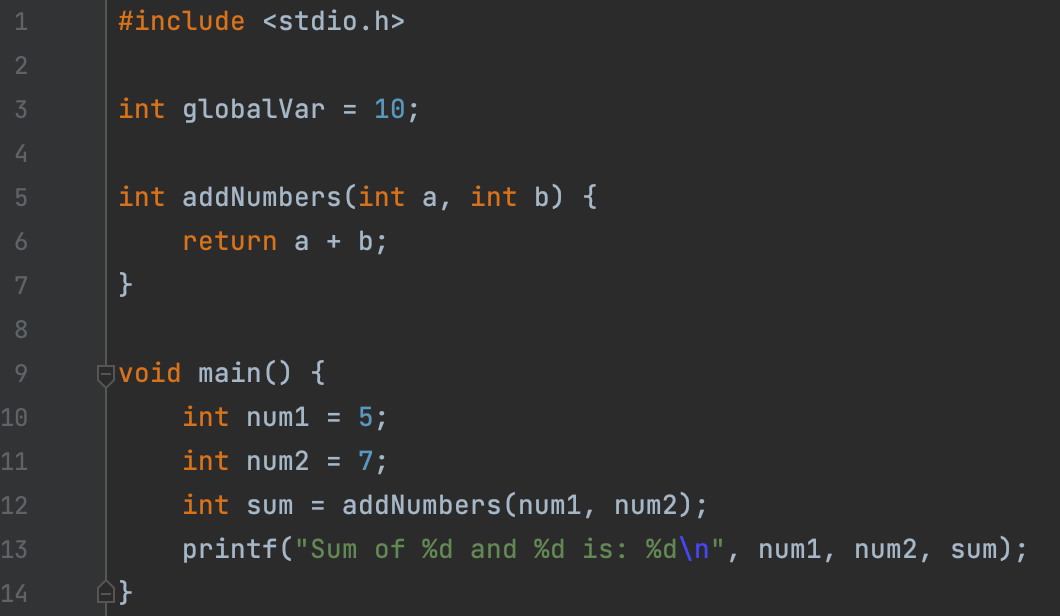
\includegraphics[width = 0.6\textwidth]{代码示例}
\caption{示例代码}
\end{figure}
这段代码由 Clang 解析生成抽象语法树后,得到的树结构如下图 2-2 所示。
\begin{figure}[h]
\centering
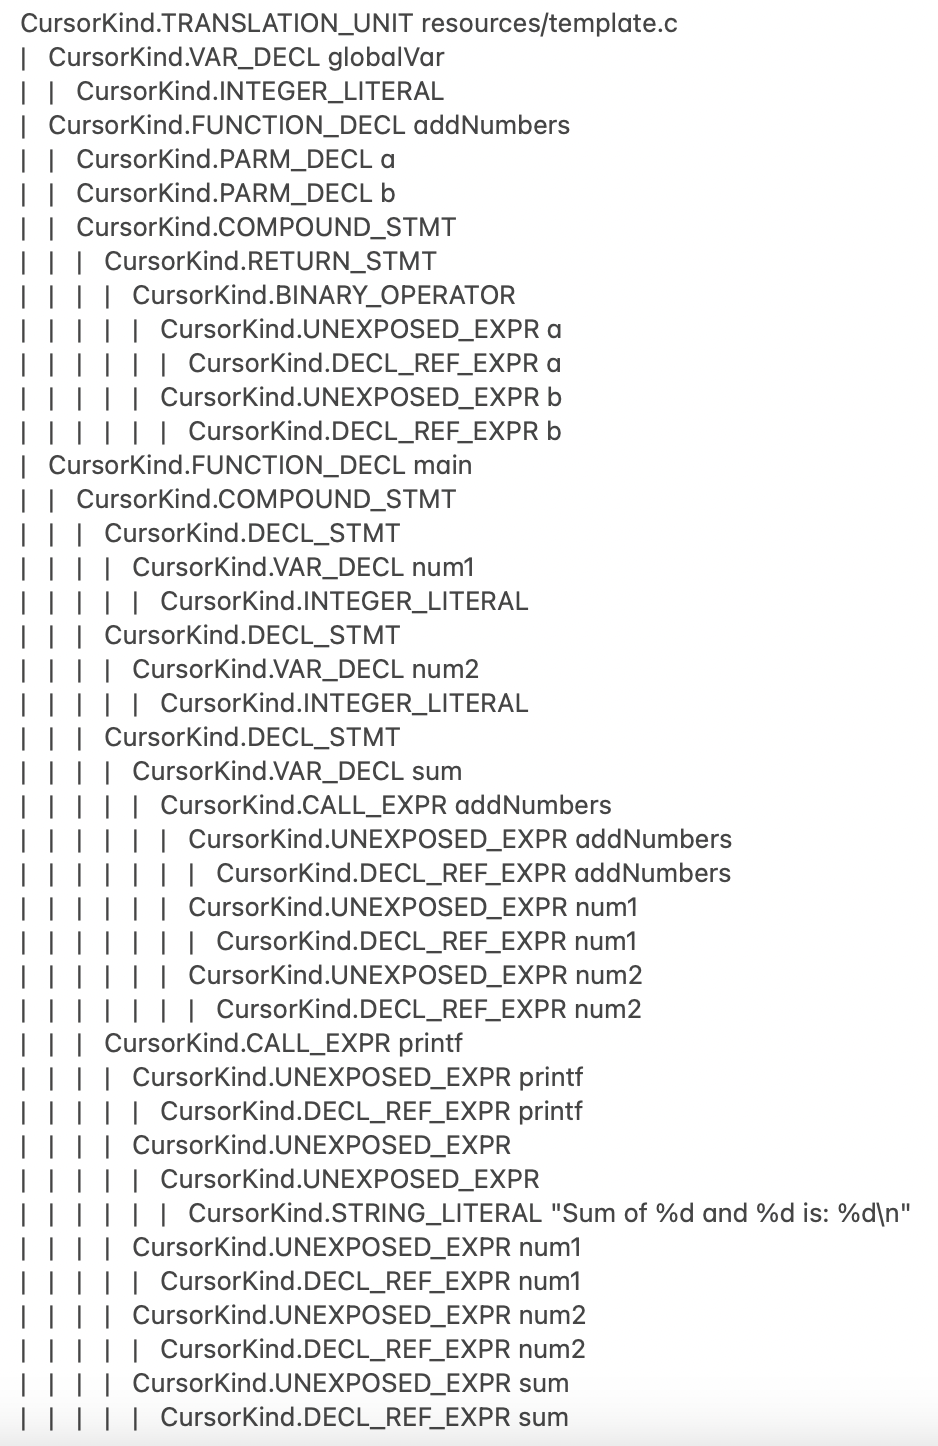
\includegraphics[width = 0.6\textwidth]{ast示例}
\caption{示例代码对应的抽象语法树结构}
\end{figure}

在 libclang 解析得到的抽象语法树中,游标(cursor)是一个核心概念,它作为一个
指针或引用存在,每个 cursor 都与 AST 中的一个特定节点相对应,表示了源代码中的
一个结构元素。通过操作 cursor,可以遍历整个 AST,访问和分析代码中的各种元素,
如获取变量的类型、函数的参数列表、类的成员等。libclang 提供了一系列 API 函数来
操作 cursor,例如:遍历 AST 中的 cursor、获取 cursor 的类型(如是否为方法定义、变
量定义、变量引用等)、获取 cursor 所代表的源代码元素的名称、类型、位置等信息、
获取 cursor 的父节点或子节点等。本文通过操作游标,遍历 AST,获取整个 AST
的结构。


Clang 定义了一套节点类型标识。AST 的顶层节点类型是Translation\_Unit标签,表
示一个翻译单元,对 AST 树的遍历,实际上就是遍历整个 Translation\_Unit。Function\_Decl
指的是函数定义,在 clang 中是不区分函数声明和函数定义的,统一用 Function\_Decl
来标识,两个区分主要看是否有函数体,在 libclang 中提供了程序接口供开发者调用判断。
Parm\_Decl 是参数节点,上面的例子中,函数 addNumbers 有两个参数 a 和 b。
CompoundStmt 代表大括号,函数实现、struct、enum、for 的 body 等一般用此标签包起
来。DeclStmt 是定义语句,里边可能有 VarDecl 等类型的定义,VarDecl 是对变量的定
义。CallExpr 标签表示函数调用 Expr,子节点有调用的参数列表。ReturnStmt 表示返回
语句。






\section{方法调用链提取与分析}
本文以整个代码项目为分析对象,代码中的方法为分析单元,方法之间的调用关系则是本文的分析基础。在使用 libclang 提取代码的抽象语法树后,遍历整棵树来提取方法之间的调用关系。这部分我们重点关注抽象语法树上的方法节点,以及方法节点内部的调用节点,对应着代码中,方法的定义和方法内部对其他方法的调用。


对抽象语法树的遍历主要分为两次,第一次遍历的目的是获取所有的方法定义。首先提取所有的
FUNCTION\_DECL 节点,它表示方法的定义,在该节点中可提取方法签名。在
FUNCTION\_DECL 节点下,提取子节点 PARM\_DECL,该节点表示方法的参数列表,
在该节点中可提取参数名称和参数类型等参数相关信息。然后提取 FUNCTION\_DECL
节点的子节点 VarDecl,该节点表示在该方法内定义的局部变量。在对方法进行分析时,
我们本身不关心方法的内部实现,但是由于在 C/c++语言中,存在局部变量可以和全局
变量重名的情况,在这里提取方法内定义的局部变量,方便后续在提取全局变量时,对
变量进行作用域的判断。除此之外,还需提取整个方法的 token 序列,所在文件以及作
用域。


第二次遍历的目的是提取方法之间的调用关系。提取 FUNCTION\_DECL 节点
的子节点 CALL\_EXPR,该节点标签表示的是调用语句,可提取调用的方法名。注意,
由于主要分析该项目中由开发者定义的方法之间的依赖关系,所以对于一些标准库方法
的调用选择忽略,不进行提取。具体的计算流程如算法 2-1 所示。


\begin{algorithm}[H]
    \caption{Scan and Analyze Code Files}
    \KwIn{项目中的所有代码文件: $files$}
    \KwOut{方法摘要表: $functions$}
    \KwLine
    \SetKwFunction{FMain}{scanAndAnalyze}
    \SetKwProg{Fn}{Function}{:}{}
    \Fn{\FMain{$files$}}{
        $functions \gets \{\}$ \KwComment{$\#$ 初始化方法摘要} \;
        \KwLine
        \KwComment{$\#$ 第一次扫描:收集方法的定义} \;
        \ForEach{$file \in files$}{
            $cursor \gets \text{libclang.parse}(file).cursor$ \KwComment{$\#$ 获取AST的根cursor} \;
            \texttt{traverse(cursor, 0, functions, file, True)} \KwComment{$\#$ 遍历AST,收集方法定义} \;
        }
        \KwLine
        \KwComment{$\#$ 第二次扫描:分析方法调用情况} \;
        \ForEach{$file \in files$}{
            $cursor \gets \text{libclang.parse}(file).cursor$ \KwComment{$\#$ 获取AST的根cursor} \;
            \texttt{traverse(cursor, 0, functions, file, False)} \KwComment{$\#$ 分析方法调用} \;
        }
        \KwLine
        \KwReturn{return $functions$} \;
    }
    \KwLine
    \SetKwFunction{FTraverse}{traverse}
    \SetKwProg{Fn}{Function}{:}{}
    \Fn{\FTraverse{$node, depth, functions, filePath, isFirstScan$}}{
        \If{$isFirstScan$}{
            \If{$node.kind == CursorKind.FUNCTION\_DECL$}{
                $function \gets \text{collectionInfo}(node)$ \KwComment{$\#$ C收集方法信息} \;
                $functions.\text{add}(function)$ \KwComment{$\#$ 将方法添加到方法摘要} \;
            }
        }
        \ElseIf{$node.kind == CursorKind.CALL\_EXPR$}{
            \texttt{parse(node)} \KwComment{$\#$ 分析被调用的函数} \;
        }
        \ForEach{$n \in node.get\_children()$}{
            \texttt{traverse(n, depth + 1, functions, filePath, isFirstScan)} \KwComment{$\#$ 递归遍历子节点} \;
        }
    }
    \end{algorithm}

\clearpage
分析结束后,将会获得每个方法的方法调用链,对应于一个方法摘要表,包括项目
代码中所有的方法和方法之间的调用关系,除此之外还包括方法的参数表、方法主体和
所在文件等其他信息。

\section{全局变量定义-使用链提取与分析}
在C/c++代码中,全局变量的定义、作用域、生命周期和方法是类似的,所以在本文中,将全局变量也作为独立的代码单元进行分析。
全局变量定义-引用链的提取和方法的定义和调用提取类似,对 AST 的遍历主
要也分为两次。具体流程如图2-3。

\begin{figure}[h]
\centering
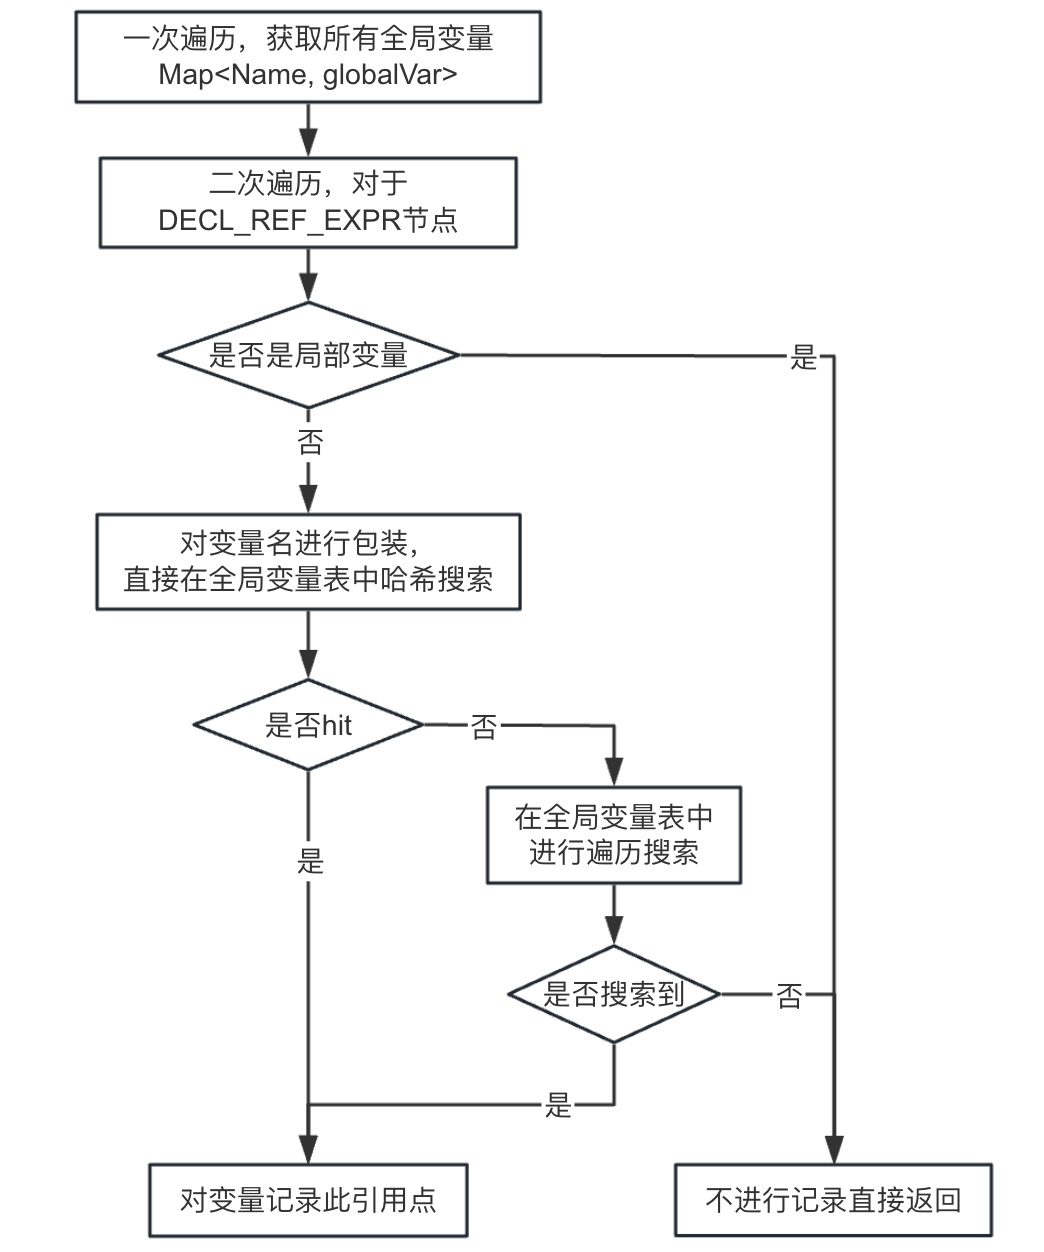
\includegraphics[width = 0.7\textwidth]{全局变量提取流程图}
\caption{示例代码对应的抽象语法树结构}
\end{figure}

第一次遍历获取所有的全局定义。首先提取所有的
VAR\_DECL 节点,它表示变量定义,然后提取节点中的变量名和变量类型。注
意,由于在 AST 中的节点标签中无法区分变量是否是全局的,所以这里根据节点在 AST
中的深度来判断是否是全局变量,并且在变量名前加上针对该项目文件的绝对路径,来
保证变量名的唯一性。在确定其为全局变量后,还需进一步提取该变量的作用域。在
C/c++语言中,static关键字可用于修饰变量和方法,意味着该变量或该方法只能在其所在文
件内使用,而不是全局可用,因此需要对其作用域进行判断。一次遍历提取到的结果是
一个全局变量表,这里使用哈希表 Map<Name, globalVar>的数据结构进行存储,方便对
全局变量进行查找。

第二次遍历的主要目的是提取全局变量的引用点。在方法节点子树中搜索
DECL\_REF\_EXPR 节点,该类型节点表示对变量的引用,这里首先判断被引用的变量是否是局部
变量,根据方法摘要表中该方法的相关信息可以判断,如果是则直接返回,因为我们不关心方法内的局部变量引用。如果不是,则证
明使用的是全局变量,首先在哈希表中进行查找该变量名,以节省检索时长,如果查找到了,说明
是在该文件中定义的全局变量,同时能够保证被 static 修饰的全局变
量的判断的准确性。如果没有查找到,则说明引用了别的文件中定义的全局函数,则在哈希
表中进行遍历查找,记录该全局变量被引用的方法。具体提取流程如图 2-3 所示。

分析结束后,则获得了每个全局变量的定义-引用链,对应于一个全局变量信息表,
包括项目代码中所有的全局变量和变量的引用点,除此之外还包括全局变量的类型、作
用域和所在文件等其他信息。

\section{基于方法特征的代码度量提取}

代码内聚度和代码耦合性是衡量软件设计质量的两个核心指标,它们直接反映了代
码质量。代码内聚度指的是模块(如函数、类或组件)内部元素之间的相关性。高内聚
度意味着模块内的所有元素都紧密地围绕着一个单一的、明确的功能,代码更容易理解
和维护[9]。代码的耦合性则描述了模块之间的相互依赖。低耦合度意味着模块之间的依
赖关系最小化,每个模块都可以独立地执行其功能,而不需要过多地依赖其他模块。低
耦合度的代码更容易测试和维护[10]。


基于方法摘要和全局变量信息表,我们计算如下代码度量,用于分析代码质量。


\subsection{基于内聚度缺乏度的内聚性分析}

LCOM(Lack of Cohesion in Methods)系列指标是根据模块内聚度的缺乏程度来衡量模块的内聚度的指标。在本文中,
面向对象语言以类为研究范围进行计算内聚度,非面向对象的语言以文件为研究范围进
行计算,类中的成员属性对应文件中的全局变量,类中的成员方法对应文件中定义的方
法。LCOM 指标的核心思想是度量一个类中方法对实例变量(属性)的共享程度。不同
版本的 LCOM 有着不同的计算方法和含义,体现了不同的侧重点。这里一共计算以下四个指标:


(1)LCOM1,含义是不引用相同字段的方法对数目[11]。计算公式如式(2-1)
\begin{equation}
    {LCOM1}=\left\{
        \begin{array}
        {c}P-Q,  ifP\geq Q \\
        0,  otherwise
        \end{array}\right.
\end{equation}

其中,P 是不共享实例变量的方法对的数量,Q 是共享实例变量的方法对的数量。
如果 LCOM1 的结果为负数,则被置为 0。
在计算时,对于每个文件首先构建方法耦合图(method coupling graph),将提取到
的方法作为图中节点,对方法两两进行判断,如果两个节点都引用相同的字段,则它们
之间用一条无向边连接,按式(2-2)计算,
\begin{equation}
LCOM1 = choose(n,2)-e
\end{equation}

其中 n 是文件中的方法总数,e 是图中的实
际边数,即图中可能的最大边数减去实际的边数,得到的值即为 LCOM1

(2)LCOM2,含义是不引用相同字段方法对与引用相同字段方法对数之差[12]。
LCOM2相比于LCOM1,考虑到了类中所有方法和变量的相互作用,其计算公式如式2-3:
\begin{equation}
{LCOM2}=\frac{1}{{a}}{\sum(a-m_{a})}
\end{equation}
其中,\(a\)是类中属性的数量,\( m_a \)是访问属性\(a\)的方法数量。
在计算时,首先构建方法属性图(method-attribute graph),将提取到的方法和全局
变量作为图中节点。如果方法引用了变量,则有一条有向边从方法节点指向属性变量,
计算公式如式2-4,
\begin{equation}
{LCOM2} = 1 - \frac{e}{n \times a}
\end{equation}
其中 \(n\) 为方法数,\(a\) 为变量数。假设 \(e\) 是图中的实际边数,得到的值即为 LCOM2。

(3)LCOM3,含义是以方法为顶点,两方法引用相同字段则有边构成的无向图的连通
分支数[12]。
LCOM3 是对 LCOM2 的进一步改进,其计算公式如式2-5:
\begin{equation}
{LCOM3=(\frac{\sum_{i=1}^n(m_i-a_i)}{m})-a}
\end{equation}
其中,\(m\)是方法的数量,\(a\)是变量的数量,\( m_i \)是第 i 个方法访问的属性数
量,\( a_i \)是被第 i 个方法访问的属性数量。LCOM3 试图通过分析方法和属性之间的关系
来提供更细致的内聚度度量。

实际计算时,如式2-6,基于上述计算出的 LCOM2 指标可以快速地计算出 LCOM3
\begin{equation}
{LCOM3} & = & \frac{n}{n-1} \times {LCOM2}  & = & \frac{n - \frac{e}{a}}{n-1}
\end{equation}

(4)LCOM4,含义是以方法为顶点,两方法引用相同字段或有调用关系则有边构成无
向图的连通分支数[13]。

计算时,构建方法耦合图,节点是方法。如果两个节点都引用相同的字段,则它们
之间用一条无向边连接,除此之外,如果两个节点有调用关系,则也用一条无向边将它
们连接。根据深度搜索的方式,计算图中的连通分支数,得到的值即为LOCM4.

\subsection{基于连通性的内聚性分析}
TCC(Tight Class Cohesion)和 LCC(Loose Class Cohesion)是用于衡量模块内
聚度的指标,这两个指标主要关注于模块中方法之间的连通关系,核心思想是通过
分析模块中方法如何相互作用以及如何访问共同资源(如全局变量)来评估模块的内聚度。


(1)TCC,含义是有连通关系的方法对数与总方法对数的比值[14]。
TCC 关注于模块中方法之间的“直接连接”。如果两个方法直接共享访问同一个变
量,则认为这两个方法是直接连接的。计算时,对于每个文件首先构建方法耦合图,对
方法两两进行判断,如果两个节点都引用相同的字段,则它们之间用一条无向边连接,
计算公式如式2-7,其中\(n\)是文件中的方法总数,\(e\)是图中的实际边数
\begin{equation}
{TCC} = \frac{e}{choose(n,2)}
\end{equation}

(2)LCC,基于方法间接引用共同字段关系的传递闭包计算[14]。
LCC 除了考虑直接连接的方法对外,还包括了间接连接的方法对。如果两个方法不
是直接连接,但可以通过一系列的方法调用来连接,则认为它们是间接连接的。LCC 的
值基于模块中直接或间接连接的方法对占所有可能方法对的比例来计算。因此,LCC 的值
通常不低于 TCC 的值,并且提供了一个更宽泛的模块内聚度视角。


计算时,对于每个模块首先构建方法耦合图,对方法两两进行判断,如果两个节点
都引用相同的字段,则它们之间用一条无向边连接表示直接连接,如果方法之间有调用,
则也将方法进行连接,并连接当前节点和调用节点的所有邻居节点。计算公式如式 2-8,

\begin{equation}
{LCC=e+\frac{e_{indirect}}{choose(n,2)}}
\end{equation}
其中\(n\)是文件中的方法总数,\(e\)是图中的直接连接边,\(e_{indirect}\)是除直接连接边的边数。


\subsection{方法间耦合性分析}

耦合是在软件架构中用来描述模块间相互依赖和连接程度的一个重要指标。耦合度的高低直接影响到系统的维护性和可扩展性。在现有的研究和实践中,耦合度通常被细分为六个等级,这些等级从高到低反映了模块间依赖的紧密程度。本文关注的是方法与方法之间的耦合性,方法间的耦合性反映了不同方法之间的依赖关系,它直接影响代码的可读性、可测试性以及后续的维护和扩展。通过深入分析方法级别的耦合性,研究方法如何通过参数传递、调用关系、共享全局变量等方式相互依赖,我们可以更准确地识别潜在的设计缺陷和优化机会,从而提高系统的模块化程度,增强系统的可维护性和可扩展性。

\begin{table}[htbp]
\caption{软件架构中耦合性分类}
\vspace{0.5em}\centering\wuhao
\begin{tabular}{ccccc}
\toprule
耦合性类别 & 描述 & 耦合程度 & 本文是否分析 \\
\midrule
内容耦合 & 模块直接访问或修改另一个模块的内部数据 & 6 & 否\\
公共耦合 & 模块访问同一公共数据环境 & 6 & 是 \\
外部耦合 & 模块共享全局简单数据结构 & 4 & 是 \\
控制耦合 & 模块传递控制信息,影响计算流程 & 3 & 是 \\
标记耦合 & 通过参数传递复杂数据结构信息 & 2 & 是 \\
数据耦合 & 通过参数传递简单数据 & 1 & 是 \\
\bottomrule
\end{tabular}
\end{table}


内容耦合是耦合度最高的一种形式,它表示一个模块能够直接访问或修改另一个模块的内部数据和结构。在方法级的耦合分析中,这种耦合形式通常不被考虑,因为方法间的直接数据访问往往通过参数传递或者 API 调用实现,而不是直接的内容访问。

公共耦合发生在多个模块共同访问某个全局数据环境时。这种数据环境可能是全局数据结构、全局变量或内存公共区域等。在提取到的全局变量表中,对于复杂数据结构如结构体和数组,其引用点所在的方法之间均存在公共耦合关系。


外部耦合与公共耦合相似,但区别在于它涉及的是对全局简单变量的访问。例如,当多个模块访问或修改相同的全局简单类型变量时,则这些模块之间存在外部耦合。


控制耦合指模块之间传递信息中包含用于控制模块内部的信息。在提取到的方法摘
要表中,遍历方法,如果该方法调用其他方法时,对应方法的参数列表中有变量决定了
被调用方法中的计算流程,则方法之间存在控制耦合关系。


标记耦合指通过参数表传递数据结构信息,调用时传递的是数据结构。在方法摘要
表中提取了方法的参数列表,包括参数名和参数类型,根据参数类型,可以确定
参数表中是否包含复杂类型。除此之外,在方法的调用表中,也提取了方法调用的
函数,结合这两个信息,即可确定两个方法是否存在着标记耦合关系。


数据耦合指通过参数表传递简单数据。与标记耦合类似,根据参数类型可以确定参
数是否全部为基本类型,结合方法调用表,即可确定两个方法是否存在数据耦合。
\subsection{方法扇入扇出度量分析}

方法的扇入(Fan-in)和扇出(Fan-out)是软件工程中用于衡量方法复杂性和模块
间依赖关系的两个指标。


扇入是指调用某个方法的不同方法的数量。它表示了一个方法对其他方法的依赖程
度。扇入值较高的方法通常被认为是重要的或核心的,因为它们被多个其他方法所依赖。
高扇入值可能意味着该函数执行了一个基础或共享的任务。


扇出是指某个方法直接调用的不同方法的数量。它表示了一个方法对其他方法的影
响程度。扇出值较高的方法可能更复杂,因为它们需要管理和协调更多的方法调用。高
扇出值可能意味着该方法具有较高的责任度,且可能更难以理解和维护。

\begin{figure}[h]
\centering
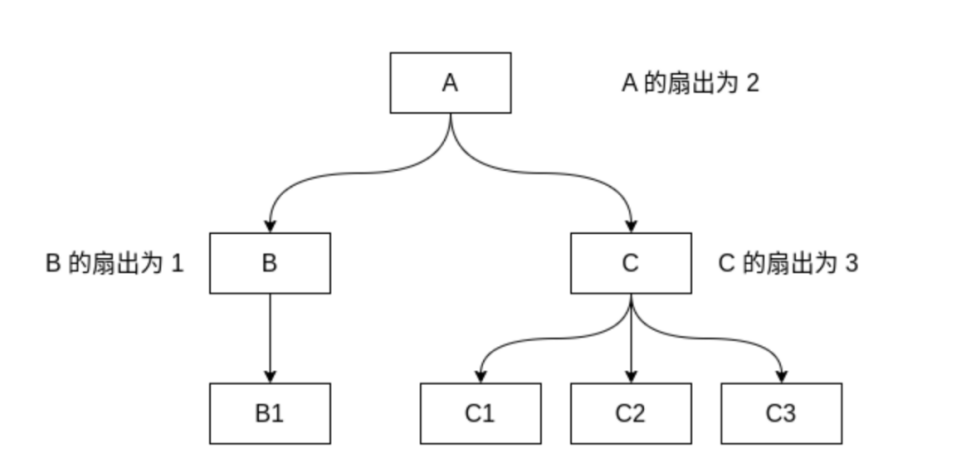
\includegraphics[width = 0.8\textwidth]{扇入扇出.png}
\caption{扇入扇出示例图}
\end{figure}

本文中对于提取到的方法摘要表,遍历每一个方法,统计其调用方法的数量即可计算出该
方法的扇出值,再以该方法名在方法摘要表中搜索调用了该方法的方法,统计总数,得
到的值即为扇入值。

\subsection{结合静态检测工具提取缺陷}

为了更准确地衡量代码质量,本文结合了静态代码分析工具 Cppcheck,对项目中的源代码进行了全面的检测和分析。Cppcheck 是一款开源的静态分析工具,专门用于检测 C/C++ 代码中的潜在错误和编码规范问题。它通过静态分析技术,扫描源代码,识别可能存在的内存泄漏、空指针解引用、未初始化变量等常见问题,并提供详细的诊断报告。与传统的编译器警告不同,Cppcheck 不依赖于程序的编译过程,它直接分析源代码的结构和逻辑,从而能够发现更广泛的潜在问题,尤其是那些难以通过常规测试手段捕捉到的错误。

在本研究中,Cppcheck 的检测结果被视为代码质量评估的重要组成部分。通过集成 Cppcheck,我们不仅能够评估代码的功能性和正确性,还可以进一步揭示代码中潜在的安全隐患和性能瓶颈。检测结果中包括了诸如错误、警告和建议等不同级别的信息,这些信息帮助开发者识别代码中的潜在问题并及时修复,进而提高代码的可维护性和健壮性。

此外,Cppcheck 提供的报告与其他度量指标(如内聚度、耦合度等)相结合,共同构成了全面的质量评估体系。用户可以根据检测报告对代码质量进行更细致的判断和分析,从而为后续的优化和重构提供科学依据。通过这种方式,本研究实现了对代码质量的多维度综合评价,为开发者提供了更为精确的质量检测和改进方向。


\section{实验结果与分析}

\subsection{实验数据描述与分析}
本文收集了表2-2中所示的软件项目为示例项目,这些项目在github上的收藏数均在千以上,说明这些项目在开源社区中有着一定的影响力,使用范围比较广泛。除此之外,这些项目有着比较活跃的社区,说明其还在不断更新迭代过程中,所以能提供较为丰富的变更历史,以供后续的实验分析。

\begin{table}[htbp]
\caption{示例项目}
\vspace{0.5em}\centering\wuhao
\begin{tabular}{cp{10cm}c}
\toprule
项目名称 & 项目简介 & 收藏数 \\
\midrule
antiword & 用于提取 Microsoft Word 文档内容的工具 & 13k\\
librdkafka & Apache Kafka 的 C/C++ 客户端库,用于与 Kafka 集群
进行通信 & 18k \\
TheAlgorithms & 各种算法的开源实现的集合,涵盖了计算机科学、数学和统计学、数据科学、机器学习、工程等各种主题 & 57k \\
libbpf & linux 内核观测技术的一个脚手架库 & 1.9k \\
FFmpegKit & FFmpeg 工具包 & 3.7k \\
jemalloc & 通用的 malloc(3)实现,强调碎片避免和可扩展的并发支
持 & 9k \\
\bottomrule
\end{tabular}
\end{table}

对示例项目提取基于内聚度缺乏度和基于连通性的内聚度指标、耦合性以及扇入扇出,这些指标一定程度上反映了代码质量。内聚度在本文中是一个模块级别的指标,它衡量一个模块内部各个组件(本文中是方法和全局变量)之间关系的紧密程度的指标。内聚度高的模块意味着模块内的各个部分紧密合作以完成某一特定任务,模块的职责单一,功能聚焦。本文中计算了两类共六种内聚度指标,在同一项目中,人工检查每种内聚度在最差的前5\%的模块,判断是否能被开发者接受,以此来验证内聚度指标的有效性。

对于耦合性,本文中提取了五种不同的耦合类别,每种类别的耦合程度并不相同,数据耦合、标记耦合、外部耦合、公共耦合,耦合程度依次递增。这里对于耦合性的判别标准需要根据是否在同一个模块进行区分。对于同一模块内,代码往往有共同的上下文和职责范围,因此要求尽量采用数据耦合,因为通过参数传递数据,方法的输入输出明确,易于测试和维护;允许标记耦合和外部耦合,允许通过传递数据结构优化参数列表简洁性;减少公共耦合,模块内共享状态可提高效率,但要避免复杂的依赖关系。对于不同模块的方法,则要求尽量采用数据耦合,数据耦合方法之间的独立性强,模块职责单一,代码易于测试和复用;减少标记耦合,优化接口设计,避免通过标记变量传递复杂的变量;杜绝公共耦合、外部耦合:避免全局变量的滥用,防止影响模块之间的依赖关系和模块内部的可测试性。同样也是通过人工检验不符合要求的耦合性,判断是否能被开发者接受,以此来验证耦合性指标的有效性。

对于扇入扇出也是类似的,传统要求尽量高扇入低扇出,高扇入表示其他模块依赖该模块,模块的功能可能是系统中其他模块的核心或基础,复用性较好;低扇出表示该模块没有过多地依赖其他模块,因此它具有更高的独立性,更易维护。这里也是通过人工检查两种指标在最差的前5\%的方法,判断是否能被开发者接受,以此来验证扇入扇出指标的有效性。

为了更准确地衡量代码质量,本文结合了静态分析工具 Cppcheck,对项目代码进行了检测。检测结果作为质量评估的一部分,提供给用户进行判别。

接受率指标计算公式如式2-9
\begin{equation}
{AR} = \frac{A}{T} \times 100\%
\end{equation}
其中AR表示接受率,A表示开发者接受的不符要求的示例数,T表示方法检测到的不符要求的样例数。




\subsection{实验结果与分析}
1. 内聚度接受率实验结果及分析

(1)内聚度接受率实验结果

对示例项目人工检验得到的接受率进行统计,得到的结果如表2-3。

\begin{table}[htbp]
\caption{内聚度接受率}
\vspace{0.5em}\centering\wuhao
\begin{tabular}{ccccccc}
\toprule
项目名称 & LCOM1 & LCOM2 & LCOM3 & LCOM4 & TCC & LCC \\
\midrule
antiword & 91.3 & 84.2 & 84.2 & 91.3 & 84.2 & 84.2 \\
librdkafka & 73.7 & 73.7 & 73.7 & 73.7 & 78.4 & 78.4 \\
TheAlgorithms & 89.2 & 74.9 & 74.9 & 89.2 & 74.9 & 74.9 \\
libbpf & 87.3 & 83.4 & 87.3 & 87.3 & 93.7 &  93.7 \\
FFmpegKit & 71.3 & 69.2 & 74.9 & 76.6 & 89.3 & 84.9 \\
jemalloc & 82.2 & 82.2 & 82.2 & 82.2 & 88.6 & 88.6 \\
\bottomrule
\end{tabular}
\end{table}
对于内聚度的接受率,经过分析可以发现指标基本都在70\%以上,表现良好。通过对比,发现在antiword、TheAlgorithms等比较简单的项目中,内聚度在6项指标中常出现相同的接受率,经过分析发现这是因为在同一项目中,尽管6项指标的计算方式和侧重点都不同,但是最差的前5\%基本上是重合的,这意味着一个模块如果在LCOM1中表现的很差,在其他指标中也通常表现得很差,这符合通常认知,同时也侧面验证了指标的准确性。但是对于FFmpegKit等较复杂的项目,6项指标则不太相同,体现了不同内聚度计算方式的侧重点。

2. 内聚度接受率实验结果实例分析

对内聚度实验结果进行进一步分析,这里选取 antiword 项目中的内聚度表现最差的模块 misc.c 文件进行分析,该文件作为一个模块来进行内聚度的计算。为了更好地理解这一现象,进一步检查了该模块的源代码,并对其结构进行了统计分析。具体来看,misc.c 文件中一共定义了 1 个全局变量和 15 个方法,其中 11 个方法并未被同一模块内的其他方法调用,只有 3 个方法之间存在相互调用关系,而仅有 2 个方法使用了该模块定义的全局变量。

通过分析可以发现,尽管该模块包含了一定数量的方法和变量,但模块内各个方法和变量之间的依赖关系极为薄弱。大部分方法相互之间没有调用关系,且仅有少数方法与全局变量发生交互。这样的结构表明,模块内的功能划分较为松散,各个功能单元之间缺乏必要的协作和紧密联系。因此,该模块的内聚度较差,功能的集中性和一致性较低,导致其内聚度值显著较低。因此,通过对 misc.c 文件内聚度的分析,我们不仅可以得出该模块的内聚度较差的结论,还能为未来的重构和优化提供指导意见。例如,增强模块内部方法之间的调用关系,优化变量的使用方式,以提高模块的内聚度,从而提升系统的整体质量和可维护性。

2. 其他度量接受率实验结果及分析

对示例项目人工检验得到的接受率进行统计,得到的结果如表2-4。

\begin{table}[htbp]
\caption{其他度量接受率实验结果}
\vspace{0.5em}\centering\wuhao
\begin{tabular}{cccc}
\toprule
项目名称 & 耦合性接受率 & 扇入扇出接受率 & 静态工具缺陷接受率 \\
\midrule
antiword & 84.2 & 56.4 & 100.0 \\
librdkafka & 73.7 & 43.3 & 98.8 \\
TheAlgorithms & 99.2 & 87.6 & 100.0 \\
libbpf & 78.3 & 42.1 & 100.0 \\
FFmpegKit & 64.0 & 43.3 & 94.6 \\
jemalloc & 87.8 & 43.3 & 100.0 \\
\bottomrule
\end{tabular}
\end{table}

从实验结果来看,不同项目在各项度量指标上的接受率存在一定差异。大部分项目的耦合性接受率较高,而扇入扇出的接受率普遍较低,大部分的项目上只达到了40-50\%的水平,而所有项目对静态工具检测出来的缺陷上的接受率都较高,说明静态工具的可靠性较好。接下来对所有指标的实验结果进行进一步分析。

(1)耦合性接受率分析

首先分析耦合性,耦合性的接受率在几个项目中的表现不尽相同。对于结构较为简单的项目,如antiword和jemalloc,接受率均能达到较高的水平,在TheAlgorithms项目上甚至能达到99\%以上的接受率,这是因为简单项目结构较为简单,各个模块功能明确,职责单一,所以耦合性不良的样例很少,维护起来也更加容易,尤其对于TheAlgorithms,这个项目是对各种算法的开源实现,模块和模块之间几乎不存在相互依赖和调用的情况,每种算法独立开发,实际上是库函数,仅在需要时供开发者调用。而在复杂项目中,如FFmpegKit,耦合性接受率相较其他项目低一些,这是由于对与大型、复杂的软件项目来讲,各模块和方法之间的依赖关系可能已经非常复杂,需要大量时间来理解现有结构并分析方法间的相互影响,对于某些功能,也的确缺乏耦合性更低的实现方式,所以接受率更低。



对耦合性实验结果进行进一步分析,针对不接受的样例,这里以FFmpegKit项目中不被用户所接受的样例进行分析。在这个样例中,方法probe\_file与另外三个模块的方法发生了公共耦合,具体来讲这几个方法共同使用了fftools\_ffprobe.c文件中定义的全局变量nb\_streams,这是一个整数。而不被用户所接受的理由是,这个全局变量实际上是一个共享全局状态,它代表了流的数量,需要在不同平台上保持一致,如表中所示,需要在android、linux、apple的环境中都保持一致,才能保证程序的正确性和一致性。在这种情况下,多个方法访问并操作该全局变量是合理的,因为这种做法确保了平台间的一致性。

\begin{table}[htbp]
\caption{其他度量接受率实验结果}
\vspace{0.5em}\centering\wuhao
\begin{tabular}{cp{12cm}}
\toprule
共同访问变量 & 方法名 \\
\midrule
\multirow{4}{*}{nb\_streams} & ffmpeg-kit/apple/src/fftools\_ffprobe.c@probe\_file \\
                              & ffmpeg-kit/android/ffmpeg-kit-android-lib/cpp/fftools\_thread\_queue.c@tq\_alloc  \\
                              & ffmpeg-kit/linux/src/fftools\_thread\_queue.c@tq\_alloc  \\
                              & ffmpeg-kit/apple/src/fftools\_thread\_queue.c@tq\_alloc  \\
\bottomrule
\end{tabular}
\end{table}


除此之外,还有一些被拒绝的样例具有共同的特征:它们涉及的都是工具类方法。例如,在 libbpf 项目中,fail 方法作为一种工具性方法,主要用于处理程序中的内部错误并输出详细的错误信息。由于该方法的功能是对程序中的异常进行集中处理,因此它在项目中会被频繁调用。然而,尽管该方法具有重要作用,但它本身并不具备足够的独立性,难以作为一个单独的模块存在。为了避免对项目结构造成过度拆分,类似功能的工具方法通常会被归纳在一个工具类模块中,以便于集中管理和供外部调用。因此,尽管这些方法的耦合度较高,但它们在实现项目功能时是不可或缺的。通过合理组织这些工具类方法,我们能够保持系统结构的清晰与高效,同时确保错误处理等基础功能能够在项目中得以统一和有效地执行。

(2)扇入扇出接受率分析

对于扇入扇出值,可以发现在这个指标上的接受率是最低的。经过实例分析,发现大部分的项目的开发模式并不完全符合高扇入低扇出的标准。比如低扇入的模块虽然复用性低,但是更加独立,意味着它们不太依赖于其他模块的实现,因此更容易被单独测试、维护和扩展,考虑到未来软件的发展,这些低扇入的方法也可能被调用,所以不能被直接接受。

对于高扇出方法的检测结果,大部分是可以接受的,但是存在某些高扇出的模块实际上是中心化的模块,这里以antiword项目中properties.c文件的vGetPropertyInfo方法为例,该方法主要根据传入的Word版本,从文档中提取各种属性信息。该方法的扇出度为30,是项目中扇出度最大的一个,但是并未被用户所接受。其原因在于,该方法的核心结构是一个包含多达9种不同情况的 switch 语句,每种情况又细分为多个子情况。根据不同的Word版本和转换需求,方法会选择不同的处理逻辑,导致总共产生了30个方法调用。集中处理所有功能逻辑的设计思路减少了冗余代码,避免了方法调用链过长所带来的潜在性能问题,尤其是在内存栈使用方面。虽然高扇出度可能会导致一定的复杂性,但对于该方法而言,集中式的处理方式有效降低了因方法调用带来的额外开销,并优化了整体系统的效率。

(3)静态工具检验接受率分析

静态工具检验得到的代码缺陷的接受率是最高的,经过分析发现只有个别错误如头文件引用错误、变量未使用等错误等不容易被开发者所接受,因为这并不是代码本身的结构问题。

\section{本章小结}

本章主要探讨了代码中间表示的提取及其质量评估度量的生成过程。首先,本文提出了基于 libclang 工具对软件项目进行抽象语法树提取的方法,并在此基础上进一步构建了方法摘要表和全局变量信息表。随后,基于提取得到的中间表示,分别介绍了基于内聚度缺乏度和基于连通性的内聚度分析,介绍了方法间耦合性分析以及扇入扇出的提取和分析,通过这几种分析手段提取了 8 个代码质量指标和 6 种耦合关系,用于对代码质量进行全面评估。最后,本章通过一系列实验验证了所提出方法的有效性,并对实验结果较差的样例进行了深入分析,探讨了其可能的原因与改进方向。

%%%%%%%%%%%%%%%%%%%%%%%%%%%%%%%%%%%%%%%%%%%%%%%%%%%%%%%%%%%%%%%%%%%%%%%%%%%%%%%
\chapter{面向代码质量评估的变更影响分析方法研究}
\section{引言}

软件变更是软件维护和发展的关键操作。通常,对软件系统所做的更改可能会导致对系统其余部分的不良副作用或连锁反应。CIA的目标是识别涟漪效应,并防止拟议变更的副作用。变更影响分析过程的输入是变更集。在进行变更影响分析后,计算影响集。变更集是用户提出的修改请求的集合,或者是软件中要更改的元素的集合。它可以引用代码级方法、语句或变量。影响集是可能受到变更集中元素影响的元素集合。影响集中的元素可以是受变更影响的文档规范、代码和测试用例。

但是本文的目的并不是根据用户的更改识别受影响的其他代码部分,而是通过代码变更影响来反映软件的代码质量,生成代码质量报告反馈给用户,因此在本文中,变更影响分析的对象是方法,识别每一个方法更改后受影响的部分,提取这种关系,反馈给用户。

方法之间的变更影响的类型可以分为以下三种类型:

(1)有直接调用关系
这种变更影响关系是显而易见的。比如方法 funcA 调用了方法 funcB,那么当 funcB
的方法签名有所变化时,调用它的方法必须对应地修改代码才能正常调用,否则会调用
不成功,甚至直接发生编译错误。

(2)共同调用另一个方法
如当 funcA 和 funcC 同时调用了方法 funcB 时,funcA 和 funcC 之间会有变更影响
关系。这种变更影响关系实际上是类型 1 的扩展,这种情况通常是 funcB 的更改引起了
funcA 和 funcC 的同时更改。

(3)逻辑上存在变更影响关系
这种变更影响关系中,方法之间虽然没有直接的调用关系,也不共同调用某个方法,
但它们的实现逻辑或者所操作的数据之间存在某种隐含的关联。这种关系可能是由于它
们共同维护某个数据的一致性、共享某些资源或者它们的输出和输入之间存在某种预期
的联系。因此,当其中一个方法发生变化时,可能会间接影响到其他方法的行为或结果,
即使这种影响在代码的静态结构中不直接可见。

\section{基于依赖关系闭包的变更影响分析}

变更影响分析的主要目标是识别软件系统中由代码修改引发的涟漪效应,从而有效防止变更产生的副作用。这一过程旨在帮助开发者全面评估变更可能带来的直接和间接影响,并制定相应的测试与维护策略。在代码变更影响关系分析中,依赖关系传递闭包分析被广泛应用,是一种基于静态依赖关系的技术手段,能够通过识别代码模块间的关联性,精准划定受变更影响的范围\cite{2021Improving}。其核心思想是利用依赖关系的传递性,通过构建和分析依赖图,揭示所有可能受到影响的代码模块或单元。

依赖关系传递闭包分析的基本假设是,软件系统中的各个代码单元(如方法或全局变量)存在不同程度的直接或间接依赖。通过对这些依赖关系的深入分析,可以识别代码变更对系统其他部分的潜在影响。本文以方法和全局变量为基本分析单元进行变更影响分析。

(1)代码预处理

在进行代码变更影响分析之前,首先需要将源代码转化为一种可供进一步分析的程序模型。该模型通常由一组能够描述代码结构和依赖关系的数据结构组成,其目的是通过抽象化和结构化的方式,将复杂的代码逻辑转化为更易于分析的形式。本文提出的预处理模块设计基于这一需求,核心思想是以抽象语法树为基础,构建程序的调用图、全局变量信息表和方法摘要表,为后续的依赖关系分析和影响范围评估提供数据支撑。

首先,使用libclang对源代码解析生成抽象语法树。抽象语法树是一种树状数据结构,用于表示源代码的语法结构,其中每个节点对应于代码中的一种语法构造(如变量声明、函数调用等)。基于抽象语法树可以直观地捕获代码的层次结构,为进一步的依赖关系分析提供了良好的起点。在生成抽象语法树之后,进一步构建全局变量信息表和方法摘要表。全局变量信息表用于记录程序中所有全局变量的相关信息,包括变量名、定义位置,以及使用了该变量的方法的名称。通过这些信息,能够明确全局变量与方法之间的依赖关系,从而识别代码中跨模块或跨方法的依赖。方法摘要表旨在对程序中的方法进行全面的结构化描述。该表包含每个方法的签名信息(如方法名和参数列表)、定义位置(如所在文件)、方法内定义的局部变量,以及方法调用的其他方法列表。这些信息不仅可以用于分析方法间的调用关系,还可以帮助区分局部变量和全局变量,从而更精确地提取依赖关系。

这些数据结构共同构成分析所需的程序模型,为依赖关系的提取和后续的传递闭包计算提供基础支持。

(2)依赖关系图的构建

依赖关系图图的构建依赖于前述提取的全局变量信息表和方法摘要表。在构建过程中,首先需要识别代码中的直接依赖关系,包括函数调用和变量引用等。前面提取的全局变量信息表和方法摘要表已经包含了这些直接依赖关系的信息。接下来,依赖关系被形式化为一个有向图,图中的节点代表代码中的基本元素,例如方法、全局变量和其他代码单元,而有向边则表示这些元素之间的依赖关系。例如,如果方法A调用了方法B,那么在调用图中就会有一条从节点A指向节点B的有向边。通过这种方式,调用图不仅能够系统地表示代码中各个元素之间的直接依赖关系,还能为后续的变更影响分析提供结构化的图形模型。

(3)变更影响分析的执行

接下来,基于依赖关系图进行变更影响分析,实际上是对方法之间变更影响关系的全面识别与提取过程。具体而言,这一过程旨在确定哪些方法在代码变更时可能受到影响,以及这些影响的传播路径。本文基于方法和方法之间的以下两种关系RBM(relationships between methods)来识别受影响的方法集IMS(impacted method set)。
\begin{equation}
\begin{array}{l}
R B M=C A L L \cup R E T U R N \text { where } \\
(f, g) \in C A L L \Longleftrightarrow f(\text { transitively)calls } g, \\
(f, g) \in R E T U R N \Longleftrightarrow f(\text { transitively)returns into } g
\end{array}
\end{equation}

这里以方法f和方法g的关系为例,CALL方法和RETURN分别代表f和g的调用和被调用关系。

对于依赖关系图中的每个节点,我们需要计算该节点的传递闭包。传递闭包是指从某个特定节点出发,通过图中定义的依赖关系,可以直接或间接到达的所有节点的集合。换言之,传递闭包反映了节点之间的依赖链条以及影响传播的范围。为了高效地计算传递闭包,利用广度优先搜索和图可及性理论递归遍历图中的各个节点及其依赖边,进而识别出所有直接或间接依赖于某个节点的其他节点。每次从某个节点出发时,都会跟踪并记录通过依赖关系可到达的所有节点,最终形成该节点的完整传递闭包。传递闭包的具体计算公式如式3-2

\begin{equation}
\begin{array}{l}
I M S^{(N)}=I M S_{C A L L}^{(N)} \cup I M S_{R E T U R N}^{(N)} \\
I M S_{ {RETURN }}^{(N+1)}=\bigcup_{{define } \in \left(I M S_{R E T U R N}^{(N)}}-I M S_{R E T U R N}^{(N-1)}\right)} I M S({ define }) \\
I M S_{C A L L}^{(N+1)}=\bigcup_{ {define } \in\left(I M S_{C A L L}^{(N)}\right)} I M S( { define }){, define } \in \\
\left(I M S_{C A L L}^{(N)}-I M S_{C A L L}^{(N-1)}\right) 
\end{array}
\end{equation}

在变更影响分析的具体应用中,我们假设依赖图中的某个方法节点发生了变更,并按上述公式进行计算,最终得到的节点集合中,所有的节点(即方法)都与初始变更的节点存在某种直接或间接的依赖关系。这些方法可以视为受变更影响的范围,意味着它们在该方法变更后,可能会因为依赖关系的传递而受到影响。通过这一分析,我们不仅可以识别出受影响的直接方法,还能揭示出那些通过多次间接依赖而受到影响的方法,帮助开发者全面了解变更的潜在影响范围。


以图 2-5 为例,在这个例子中,一共有 4 个方法,其中方法 funcA 调用了 funcB 和
funcD,funcB 调用了 funcC。在对 funcC 进行变更影响分析时,会直接影响到 funcB,
根据依赖关系闭包,会间接影响到 funcA。所以与 funcC 有变更影响关系的方法集合为
{funcB, funcA}。

\begin{figure}[h]
\centering
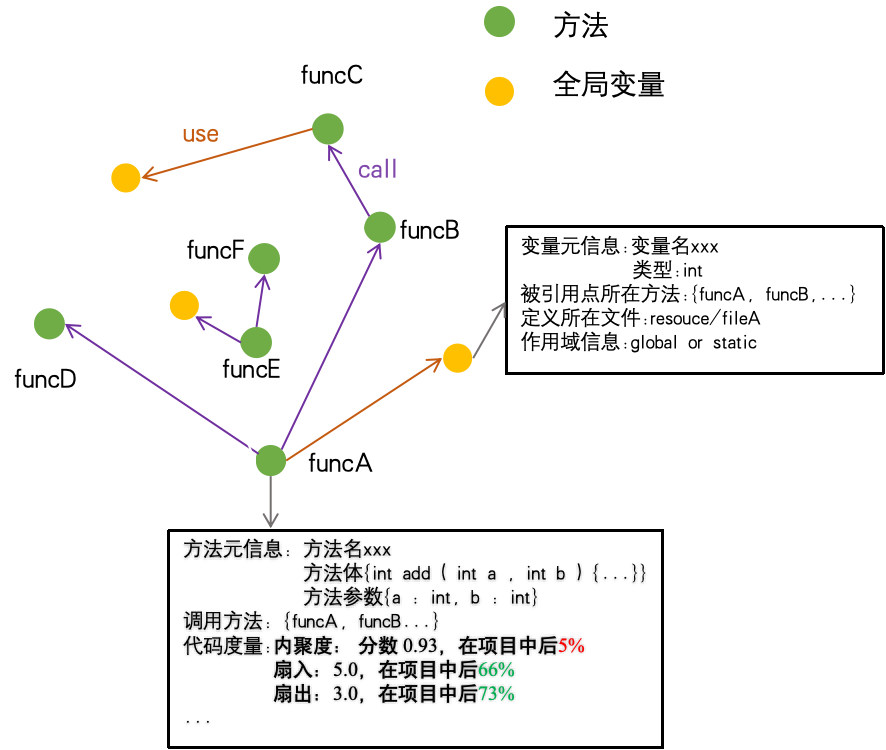
\includegraphics[width = 0.6\textwidth]{依赖关系示例.png}
\caption{依赖关系示例}
\end{figure}

\section{基于代码克隆的变更影响分析}
代码克隆(Code Clone)是指在代码中存在两段或多段内容相似或完全相同的代码片段。这些代码片段可能由于直接复制粘贴或手动修改而产生,通常是在软件开发过程中为了快速复用功能、减少重复实现或其他原因而引入的。代码克隆虽然可以在短期内提高开发效率,但在长期来看,可能对代码的维护和演化带来负面影响。

代码克隆主要分为以下三种类型:(1)完全克隆:两段代码完全相同,除了空白符、注释或格式化上的差异,这种克隆通常是直接复制粘贴的结果;(2)语法克隆:两段代码的结构和功能相同,但在变量名、函数名或字面量上存在一些简单修改。(3) 修改克隆:两段代码基本相似,但在部分语句上有较大改动。例如,某些逻辑被修改、删除或添加。这种克隆通常反映了代码的部分复用。


在代码中,克隆的代码片段是完全或部分相同的,因此它们在逻辑上往往具有相同的功能或行为。如果对其中一个克隆片段进行了变更(例如修复了一个 bug、添加了功能或进行优化),那么在其他地方相同或相似的代码也可能需要同步修改,否则可能会导致系统的不一致性或错误。

因此,本文提出了一种基于代码克隆检测的变更影响分析方法。该方法通过识别和检测软件源代码中的代码克隆,揭示了不同代码片段之间的变更影响关系。具体而言,通过检测代码克隆,可以有效地追踪在代码变更过程中,克隆代码之间的相互依赖及其潜在影响,从而为后续的代码质量分析提供了关键的依据和数据支持。这一方法不仅有助于揭示代码重复带来的潜在风险,还能为开发人员提供系统的变更影响评估,从而优化代码维护和改进的决策过程,推动软件质量的持续提升。

该方法主要分为两步,首先对源程序进行预处理,通过代码分段及代码指纹提取的方式对源程序进行编码,生成代码序列数据库。随后利用频繁模式挖掘算法得到代码克隆,具体的检测流程如图3-2所示。

\begin{figure}[h]
\centering
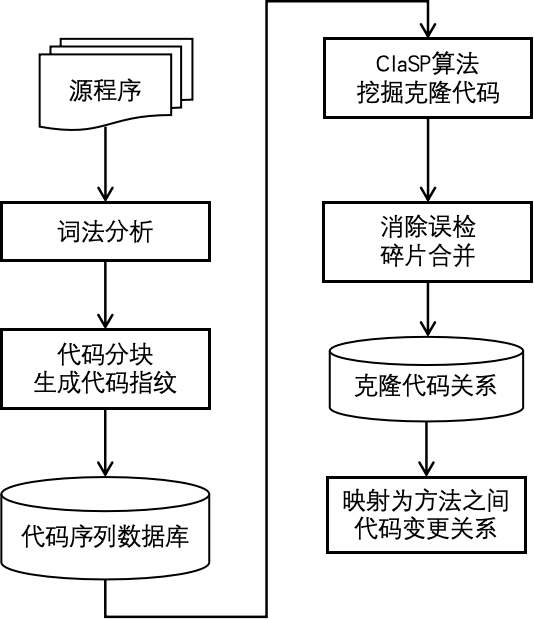
\includegraphics[width = 0.4\textwidth]{代码克隆流程}
\caption{基于代码克隆的变更影响分析方法流程}
\end{figure}



\subsection{代码预处理和分块}

为了精确有效地检测代码克隆,必须对源代码进行详细的预处理,以消除可能影响克隆检测准确性的各种干扰因素。

(1)代码标准化

首先,去除注释。注释通常用于解释代码的意图,并不直接影响程序的执行,但不同的代码实现中注释内容可能存在差异,这会导致本质相同的代码片段由于注释的不同而被误判为非克隆。因此,去除源代码中的注释是必不可少的步骤,它可以避免注释的差异干扰克隆检测的结果,从而确保算法专注于代码的实际逻辑。

接下来,去除头文件引用语句。在C/C++程序中,多个源文件往往会包含多个头文件,而不同的源文件可能引用相同的头文件。如果不对头文件进行统一的处理,算法就可能在不同的源文件中重复解析相同的头文件,进而导致无谓的计算冗余。这不仅增加了处理的时间和空间复杂度,还可能影响克隆检测的效率和准确性。因此,合理的头文件处理可以有效地去除冗余,确保分析过程的高效性。

此外,考虑到代码克隆中的语法克隆类型,变量名的标准化处理在克隆检测中具有重要意义。具体而言,为了避免因变量名的变化导致漏检,通常可以在方法内部对变量名进行统一标准化处理。即,通过将所有局部变量和参数名替换为预定义的标准变量名,从而消除变量名不同带来的影响。这一过程有助于聚焦于代码的逻辑和功能层面,而非单纯依赖变量命名的差异,从而提高克隆检测的准确性和可靠性。

通过上述预处理过程,可以生成一个清晰、标准化的源代码文件,不仅消除了无关的噪声,还确保了源代码的逻辑和结构能够被准确捕捉,为后续的克隆检测提供了高质量的输入数据。

(2)代码分块

代码分块的步骤主要目的是将代码拆解成更小、更易于对比的单元,从而提高克隆检测的准确性。其核心原因在于减少不同开发者在代码书写风格、格式和结构上的差异对检测结果的影响,确保能够准确识别功能相似或重复的代码块。

本文的代码分块策略分为几步,首先对于基本语句按固定行数分块,行数可由用户定义,默认为6行一块,行数越小则识别结果越精准,越能识别更细小的代码克隆情况。对于控制语句,识别并根据关键分块词(如 if, while, for, switch, try 等)进行分块,控制语句是代码逻辑的重要分界点,将它们作为分块的标准可以确保检测系统能聚焦于实际功能的逻辑边界,而不是因为格式的不同而导致误判。

此外,在代码克隆检测中,还需要遵循一些附加规则以确保检测的准确性和一致性。一个关键规则是大括号不被视为代码块的一部分。这一处理策略是基于实际开发中的多样化书写风格所作出的考虑:不同的开发者在代码排版上可能存在差异,例如有的开发者将大括号置于同行,而另一些则习惯将大括号另起一行。为了避免这种格式差异对克隆检测结果产生干扰,大括号被排除在代码块之外,从而确保检测过程更侧重于代码的逻辑结构,而非视觉格式上的不同。

另外,在分块过程中,为了便于后续的克隆检测和碎片合并,需要详细记录每个代码块的位置信息。这些信息通常包括:代码块所在的文件路径、代码块的起始行号和终止行号、代码块的总行数,以及每个块包含的具体行数。通过这种方式,不仅能够清晰地标识出每个代码块的位置,还能为后续的克隆碎片合并提供必要的上下文支持

通过这些步骤,代码被拆分成更小、更一致的单元,使克隆检测能够更加高效且精准地识别功能相似的代码块。

(3)代码指纹提取

这一步通过对代码的特征进行抽象和提取,从而为每个代码片段生成唯一的“指纹”,该指纹能够有效地用于识别代码片段之间的相似性或重复性。通过这种方式,不同的代码片段可以被转换为具有独特标识符的形式,从而在后续的分析中实现高效的比较和匹配。鉴于哈希算法在计算上的高效性与实现的简便性,它在生成代码指纹方面具有显著的优势。因此,本文选择采用哈希算法作为提取代码指纹的方法,以确保在保证高效性的同时,能够快速、准确地对代码进行相似性分析和重复性检测。


\subsection{基于ClaSP算法的代码克隆检测方法}
序列数据挖掘(Sequence Data Mining,SDM)是时序数据挖掘领域的一个重要研究方向,旨在从给定的输入数据库中,探索在大量对象之间随时间频繁出现的模式。判断一个模式是否具有意义的阈值被称为最小支持度。SDM 已被广泛研究,并在多个领域得到了应用,如 DNA 序列中的基序发现、顾客购买序列分析、网页点击流分析等。本文利用数据挖掘算法,提取代码克隆序列。

(1)数据挖掘领域基本概念

数据挖掘领域中有一些基本概念:

项集\cite{2013ClaSP}:设有一个集合 \( I = \{i_1, i_2, \dots, i_n\} \),其中 \( i_i \) 表示一个项。项集即为这个项的非空子集。一个项可以出现在多个项集中,但同一项集中的每个项只能出现一次,即不允许项集包含重复的项。

序列\cite{2013ClaSP}:序列是一个由项集组成的有序列表,记作 \( s = (s_1, s_2, \dots, s_n) \),其中每个 \( s_i \) 是项集。每个项集 \( s_i \) 可以进一步表示为 \( (x_1, x_2, \dots, x_m) \),其中 \( x_m \) 是项。

子序列\cite{2013ClaSP}:考虑两个序列 \( \alpha = (a_1, a_2, \dots, a_n) \) 和 \( \beta = (b_1, b_2, \dots, b_m) \),如果存在一组整数 \( 1 \leq j_1 < j_2 < \dots < j_n \leq m \),使得序列 \( (a_{j_1}, a_{j_2}, \dots, a_{j_n}) \) 是序列 \( \beta \) 的子序列,则称序列 \( \alpha \) 为序列 \( \beta \) 的子序列,序列 \( \beta \) 为序列 \( \alpha \) 的超序列。

序列数据库\cite{2013ClaSP}:序列数据库是由一组元组 \( \langle \text{sid}, s \rangle \) 构成的集合,其中 \( \text{sid} \) 为序列的标识符,\( s \) 为序列。如果序列 \( \alpha \) 是元组 \( \langle \text{sid}, s \rangle \) 中序列 \( s \) 的子序列,则称该元组包含序列 \( \alpha \)。序列数据库中包含序列 \( \alpha \) 的元组的数量被称为序列 \( \alpha \) 的支持度。

频繁子序列\cite{2013ClaSP}:给定一个正整数 \( \text{min\_support} \) 作为支持度阈值,如果序列 \( \alpha \) 的支持度大于或等于 \( \text{min\_support} \),即 \( \text{support}(\alpha) \geq \text{min\_support} \),则称序列 \( \alpha \) 为频繁子序列。所有频繁子序列的集合记为 \( FS \)。


序列支持度:记作 \( \sigma(\alpha, D) \),是指在输入数据库 \( D \) 中包含序列 \( \alpha \) 的序列的总数。如果一个模式或序列至少出现给定的用户指定阈值 \( \text{min\_support} \),即最小支持度,则称其为频繁序列。\( FS \) 是所有频繁序列的集合。频繁序列挖掘的问题就是在给定的输入数据库中,找到满足最小支持度阈值的频繁序列集合 \( FS \)。


闭合序列:如果一个频繁序列 \( \alpha \) 没有其他超序列与其具有相同的支持度,则称 \( \alpha \) 为闭合序列。否则,如果一个频繁序列 \( \beta \) 存在一个超序列 \( \gamma \),使得它们具有完全相同的支持度,则称 \( \beta \) 为非闭合序列,并且 \( \gamma \) 吸收 \( \beta \)。所有频繁闭合序列的集合记作 \( FCS \)。更正式地说,若对所有 \( \beta \in FS \),有 \( \alpha \subseteq \beta \) 且 \( \sigma(\alpha, D) = \sigma(\beta, D) \),则 \( \alpha \in FCS \)。

闭合序列挖掘的问题就是在给定的输入数据库中,找到满足最小支持度阈值的闭合序列集合 \( FCS \)。显然,频繁闭合序列的集合要小于所有频繁序列的集合。这是因为在频繁模式的集合中,很多模式可能是冗余的。例如,某些频繁模式的支持度相同,且其中一个是另一个的超序列。对于这些模式而言,冗余的超序列模式没有提供比其子序列模式更多的信息。闭合频繁模式的引入可以去除这些冗余,保留那些最具代表性和信息量的模式。

这里举例说明,表为序列数据库示例,这里设定最小支持度阈值为2。

\begin{table}[htbp]
\caption{序列数据库示例}
\vspace{0.5em}\centering\wuhao
\begin{tabular}{cccc}
\toprule
序列id(sid) & 序列 \\
\midrule
1 &  \langle (a)(ab)(bc)\rangle\\
2 & \langle (a)(abc) \rangle\\
3 & \langle (d)(a)(ab)(bc) \rangle\\
4 & \langle  (d)(ad)\rangle\\
\bottomrule
\end{tabular}
\end{table}

在这个例子中,第一个序列中有3个项集,分别是(a),(ab)和(bc),以此类推。这个例子中的闭合频繁序列\( FCS = \{ \langle (a)\rangle, \langle (d)(a)\rangle, \langle (a)(ab)\rangle, \langle (a)(bc)\rangle, \langle (a)(ab)(bc)\rangle \}\), 共5个,而频繁序列有27个。因此识别闭合频繁模式具有重要的压缩性,并且模式信息也是不丢失的。

本文中,克隆代码的指纹是一个项,每个文件是一个序列,所有文件作为序列数据库,在数据库上运行ClaSP算法挖掘所有的频繁项集,即克隆代码。

(2)ClaSP算法

ClaSP算法主要分为两步,首先生成频繁序列,作为频繁闭合的候选FCC(Frequent Closed Candidates)。第二步执行剪枝,从候选中剔除所有非闭合的序列,最终得到精确的FCS。

主要的算法流程如3-1所示

\begin{algorithm}
\caption{ClaSP算法}
\begin{algorithmic}
\KwIn{序列数据库}
\KwOut{频繁闭合序列集 $FCS$}
\State $F_1 \gets \{\text{频繁 1-序列}\}$ \\
\State $FCC \gets \emptyset$, $FCS \gets \emptyset$  \\
\For{\textnormal{all} $i \in F_1$} {
    \State $F_{ie} \gets \{\text{频繁 1-序列的长大于i的扩展序列 } \}$ \\
    \State $FCC_i \gets \text{DFS-PRUNING}(i, F_1, F_{ie})$ \\
    \State $FCC \gets FCC \cup FCC_i$\\}
\EndFor
\State $FCS \gets \text{N-ClosedStep}(FCC)$
\end{algorithmic}
\end{algorithm}


首先找到所有的频繁的1-序列(即长度为1的序列),然后,对于所有频繁的1序列,递归地调用DFS-Pruning方法来探索相应的子树(通过进行深度优先搜索)。对所有频率为1的序列进行此处理,得到FCC,最后,算法结束去除FCC中出现的非封闭序列。


\begin{algorithm}[htbp]
\caption{DFS-Pruning算法伪代码}
\KwIn{当前模式 $p$, 候选项集 $S_n$ 和 $I_n$}
\KwOut{更新后的频繁模式集 $FCC$}

$Stemp \gets \emptyset$ 
$Itemp \gets \emptyset$ 
$F_i \gets \emptyset$ 
$P_s \gets \emptyset$ 
$P_i \gets \emptyset$ \\
\If{$\neg \text{checkAvoidable}(p, I(D_p))$}{
    \For{all $i \in S_n$}{
        \If{$p' = (s_1, s_2, \dots, s_n, \{i\})$ is frequent}{
            $Stemp \gets Stemp \cup \{i\}$ \\
            $P_s \gets P_s \cup \{p'\}$ \\
        }
    }
    $F_i \gets F_i \cup P_s \cup \text{ExpSiblings}(P_s, Stemp, Stemp)$ \\
    \For{all $i \in I_n$}{
        \If{$p' = (s_1, s_2, \dots, s_n \cup \{i\})$ is frequent}{
            $Itemp \gets Itemp \cup \{i\}$ \\
            $P_i \gets P_i \cup \{p'\}$ \\
        }
    }
    $F_i \gets F_i \cup P_i \cup \text{ExpSiblings}(P_s, Stemp, Itemp)$ \\
}
\Return{$F_i$} \\
\end{algorithm}
    

在递归遍历过程中,DFS-Pruning 算法通过递归生成候选模式(包括 s-扩展和 i-扩展,分别在模式末尾和任意位置添加新元素)并检查其支持度,最终返回以当前模式 $p$ 为前缀的所有频繁模式集。算法输入包括当前频繁模式 $p$ 以及用于执行扩展操作的候选项集 $S_n$ 和 $I_n$。

在 s-扩展阶段,算法遍历 $S_n$ 中的每个候选项 $i$,检查扩展后的模式是否为频繁模式。若为频繁模式,则将其加入 $Stemp$ 和 $P_s$ 中,并通过递归调用 ExpSiblings 方法继续扩展。i-扩展部分则类似,遍历 $I_n$ 中的候选项,检查并加入频繁扩展模式到 $Itemp$ 和 $P_i$ 中,最终进行 i-扩展的剪枝处理。

最终,算法返回以模式 $p$ 为前缀的所有频繁模式集 $F_i$,其中包括通过 s-扩展和 i-扩展生成的所有频繁模式。这些操作通过递归遍历模式树,确保高效地发现所有频繁模式。


剪枝时,通过检查对应模式的子序列和超序列的支持度,将序列的节点进行合并,防止继续遍历冗余节点。最终得到的FCS即为所有克隆代码集。

(3)合并碎片

由于先前的代码分段处理导致克隆代码呈现为片段间的克隆关系,实际上这些克隆关系表现为碎片化的形式。为了恢复代码的完整性,进一步对这些碎片进行合并。具体而言,基于每段代码的位置信息,将属于同一方法的碎片进行合理整合,从而重建方法间的克隆关系。通过这种方式,最终得到的是方法与方法之间的克隆关系,反映了不同方法之间的相似性。

这种方法间的克隆关系不仅揭示了代码的重复性,还反映了不同方法之间在代码修改过程中的潜在影响。方法与方法之间的克隆关系可以被视为一种变更传播的路径,指示了某一方法的修改可能如何影响其他方法。因此,提取出的这些克隆关系实际反映和代表了方法之间的变更影响关系。

\section{基于数据挖掘的变更影响分析}
\subsection{代码变更历史提取}

在软件工程中,代码变更历史的分析是理解软件演化、优化代码质量及进行维护的重要手段之一。传统的基于依赖关系闭包的方法能够识别方法之间的浅层变更影响关系,主要侧重于语法层面和直接的依赖关系。然而,这种方法无法揭示更深层次的关系,如方法间的潜在影响和变更传播。因此,本文设计了一种基于数据挖掘技术的变更影响分析方法,主要的挖掘对象是软件项目的变更历史。该方法能够更全面、深刻地提取代码变更历史中的变更影响关系,尤其适用于具有丰富变更记录的软件项目。

该方法的核心假设是:在代码变更历史中,频繁同时更改的代码片段或方法对,通常存在着某种潜在的变更影响关系。这种变更影响关系不仅仅局限于语法上的依赖,还包括功能上的耦合和实现上的相互作用。因此,通过对这些历史变更数据的深入挖掘和分析,我们可以揭示出更深层的变更关系,为后续的代码优化、重构以及维护工作提供有力支持。

本方法的具体实现过程可以分为几个主要步骤,首先是对代码变更历史的收集与整理,然后通过数据挖掘技术提取并分析方法之间的变更影响关系。代码变更历史提取具体流程如下:

(1)收集项目代码库及变更历史记录

由于 Git 是现代软件开发中最广泛使用的版本控制工具,因此,本文的分析主要集中在 Git 项目上,如2.6.1节所示的6个项目。首先,克隆项目的代码库到本地,项目中的.git文件夹中包含了版本变更历史记录,包括所有提交(commit)记录等。每个提交代表着代码库的一次变更,包含了代码的修改、删除或新增文件等信息。通过git log命令获取每次commit的详细信息,包括每个提交的哈希值、作者、日期和提交信息等。

(2)提取每个提交的变更信息

每个提交不仅仅是一个单一的代码变更,往往涉及多个文件的更改。因此,对于每个提交,运行git show <commitHash>命令,查看该提交引入的代码变更(即“diff”或差异),这里会显示哪些文件被修改、添加或删除,本文主要关注标记为“修改”的文件,这些修改的文件中包含了具体的代码变化,即代码行的增、删、改操作,记录该commit引起的所有发生变更的代码行。

(3)定位变更代码行所属的方法

在提取了具体的代码变化后,定位这些变化的代码行所在的方法。通过libclang分析变化前文件得到的抽象语法树可获取每个方法对应的代码行,将变更的代码行的位置与方法位置进行匹配,进而得到变更的代码行所在的方法。

(4)提取变更方法与提交的关系

对于每个提交,提取出所有受影响的方法(即发生变化的方法),并将这些方法构成一个变更方法列表。这个列表反映了在特定提交中发生变更的所有方法,并为后续的变更影响分析提供了基础数据。用Map<commitID, List<Methods>>的结构存储每个commit变更的方法,作为序列数据库,便于后续分析与处理。


\subsection{基于共现关联挖掘的变更影响关系提取}

关联规则(Association Rules)是反映事物之间相互依存性和关联性的一个重要数据挖掘技术,旨在从大量数据中挖掘出有价值的项之间的相关关系。共现关系可以视为关联规则的一种表现形式,它描述了在给定集合中,某一组项(或特征)经常出现在同一事务中。例如,在零售分析中,常见的共现关系是“购买了面包的顾客通常也会购买牛奶”。在这种情况下,“面包”和“牛奶”是两个共现项。

在本文的代码变更影响分析中,共现关系描述的是在一次提交中,哪些方法经常同时发生变更。如果两个方法在多个提交中频繁一起变动,则它们之间可能存在某种依赖关系或变更影响关系。通过分析这些方法在多个提交中被频繁同时修改的情况,我们能够识别方法之间的变更影响路径,从而揭示它们的潜在关联性。

(1)频繁项集评估标准

常用的频繁项集的评估标准有支持度和置信度。
支持度表示共现项在数据集中出现的次数占总数据集的比重,于衡量一组项在数据集中的普遍程度。在代码变更分析中,支持度表示某一方法对在多个提交中同时出现的频率,计算公式如3-3.

\begin{equation}
Support(funcA,funcB)=\frac{num(AB共现)}{num(AllCommits)}
\end{equation}

置信度表示共现项中一个出现后,另一个项出现的概率。变更分析中,置信度度量当方法A被修改时,方法B被修改的概率,计算公式如3-4。

\begin{equation}
Confidence(funcA\Leftarrow funcB)=P(AB共现)/P(B出现)
\end{equation}


\section{基于深度学习的变更影响分析}

\subsection{数据集来源和收集}

当项目代码拥有丰富的变更历史时,可以通过前文中介绍的数据挖掘方法,提取具有变更影响关系的方法对。这种方法通过分析历史提交记录中方法间的共现频率,识别出在多次变更中相互依赖或相互影响的方法。然而,并不是所有软件项目都有变更历史可供我们分析,在仅有项目源代码的情况下,数据挖掘方法无法直接应用,但是只使用基于依赖闭包和基于克隆代码的方法,则无法识别除这两种关系外更深层次的变更影响。因此本文提出基于深度学习的变更影响分析方法,通过训练深度模型,对变更影响关系进行预测,以弥补另两种分析方法的不足。

为了识别那些来源除了依赖关系和代码克隆得到的代码变更影响关系,需要收集包含深层变更影响关系的方法对。而3.4节中根据数据挖掘的变更影响关系分析的方法,恰巧弥补了这一空缺。该方法可以识别出那些在多个提交记录中频繁同时发生变更的方法对,由于我们的标准设置十分严格,因此识别的变更影响关系具有较强的可靠性,可作为数据集的正例进行收集。此外,为了构建平衡的数据集,通过对项目中的方法进行随机抽样,从中选取一些不具有变更影响关系的方法对,作为数据集的负例进行收集。

在数据集收集过程中,本文面临了几个挑战。首先,一些看似活跃的项目(例如频繁提交的项目)实际上并未挖掘到大量可用数据。分析原因是由于项目规模较大,文件数量庞大,开发者的工作内容往往不具有交集,大部分的方法不会被二次更改,因此难以出现频繁的样例。其次,对于一些发展时间较长的项目,因为提交记录众多(如数万次提交),所以在收集数据时需要处理大量的提交,这使得数据处理的过程非常耗时。

为了解决这些问题,本文在选择项目时设定了一些标准。首先,优先选择规模适中的项目,这些项目既足够活跃,又不会因为过于庞大的代码库而导致数据处理困难。同时,考虑到提交记录较多的项目可能导致数据量过大,本文限制了采集范围,只选择了最近的提交记录(例如最新的10000个提交)。这一策略有两个主要考虑:一方面,确保数据量足够大,以支持后续的挖掘工作;另一方面,聚焦于那些近期频繁变动的函数,排除较为稳定且变化较少的旧函数,从而更好地反映出当前项目的活跃度和变更趋势。

最终本文选择了基于表 2-1 中列出的GitHub项目。这些项目除了符合上述条件外,还有以下优点。首先,它们的收藏数均在千以上,表明这些项目在开源社区中具有较高的关注度和影响力,并且被广泛使用。其次,这些项目的社区非常活跃,说明项目持续更新和迭代,保证了具有较为丰富的变更历史,能够为我们的变更影响关系分析提供丰富的数据支持。

\subsection{基于代码预训练模型的变更影响关系预测}

基于深度学习的影响关系预测任务的输入为两个方法体,输出为一个介于 [0, 1] 之间的值,表示这两个方法之间存在变更影响关系的概率。该概率越接近 1,表明这两个方法之间有关系的可能性越大。

考虑到代码理解的复杂性与深度,本文采用了基于预训练模型的代码表示学习方法,选择了 CodeBERT 作为核心模型。CodeBERT 是一种专为程序代码设计的预训练语言模型,通过大规模的代码语料库预训练,能够学习到代码中的丰富语法结构和语义信息。经过 CodeBERT 模型的表示学习,所得到的向量不仅包含了每个方法体的语法特征,还能够编码代码中的语义关系及其他潜在的编程特征。模型架构如图3-3所示。

\begin{figure}[h]
\centering
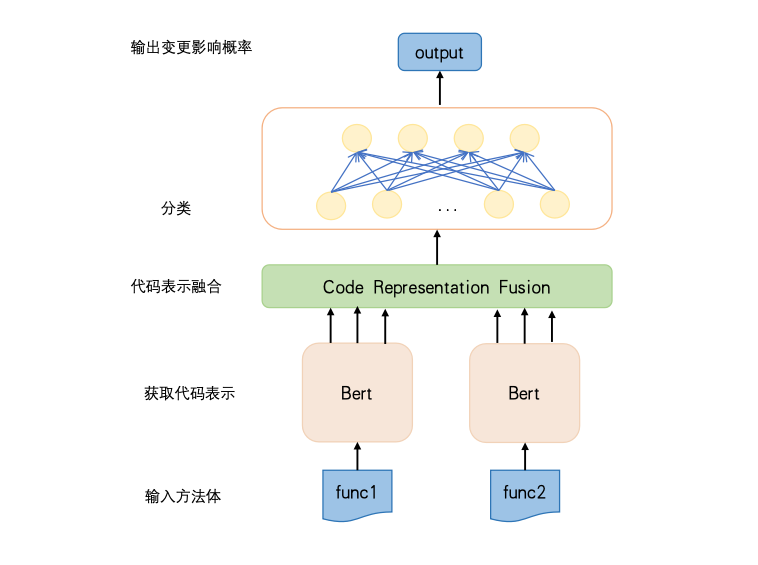
\includegraphics[width = 0.8\textwidth]{模型架构3.jpg}
\caption{基于代码预训练的深度学习模型架构}
\end{figure}


首先,将两个方法体$ F_a, F_b$,先通过代码预训练模型进行编码

\begin{align}
H_a=&Encoder(F_a) \in \mathbb{R}^{(len,dim)} \\
E_a=&mean(H_a[1:...]) \in \mathbb{R}^{(dim)}
\end{align}

得到方法的向量化表示$ E_a, E_b$,通过拼接融合这两个向量,将融合后的向量表示送入一个由两层组成的多层感知机(Multilayer Perceptron,MLP)中,再通过 softmax 层进行分类处理,将模型的输出转化为一个概率分布,表示两个方法体之间存在关系的概率。

\begin{align}
E_{a,b}=Concat(E_a,E_b)& \in \mathbb{R}^{(dim*2)} \\
logits_{a,b}=MLP(E_{a,b})&=FFN(ReLU(FFN(E_{a,b}))) \\
FFN(x)&=Wx+b\\
ReLu(x)&=max(0,x)\\
logits_{a,b}& \in \mathbb{R}^{(2)}
\end{align}

最后与真实标签计算交叉熵损失,得到loss,计算梯度,优化模型参数
\begin{align}
loss=CrossEntryLoss(logits_{a,b}, Label)
\end{align}

\section{实验结果与分析}

\subsection{实验数据集描述}

本章依旧使用表2-2的示例项目进行研究。基于深度学习的变更影响分析方法的数据集收集方式如3.5.1节所述。数据集统计信息如表3-2所示,共7351对数据,按照训练、验证、测试集 为 6:2:2 进行训练和测试。这里排除了antiword项目,因为该项目并没有官方维护的github仓库,因此无法获得足够的历史变更。

\begin{table}[htbp]
\caption{数据集统计信息}
\vspace{0.5em}\centering\wuhao
\begin{tabular}{cccc}
\toprule
项目名称 & 正例对数 & 负例对数 & 总对数 \\
\midrule
librdkafka & 1164  & 1000 & 2164 \\
TheAlgorithms & 110 & 1000 & 1110 \\
libbpf & 418 & 1000 & 1418 \\
FFmpegKit & 18 & 1000 & 1018 \\ 
jemalloc & 641 & 1000 & 1641 \\
总计 & 2351 & 5000 & 7351 \\
\bottomrule
\end{tabular}
\end{table}

\subsection{实验设置与评价方式}
1. 实验设置

(1)深度学习实验设置

针对基于深度学习的变更影响分析方法。本文使用了CodeBERTa-small-v1和codebert-base-mlm两个模型分别作为代码表示学习模型,得到的代码表示为768维,融合时使用的MLP的每层维数为(768*2,64,2)。

模型的参数设置如表3-3。

\begin{table}[htbp]
\caption{模型参数设置}
\vspace{0.5em}\centering\wuhao
\begin{tabular}{cccc}
\toprule
超参数 & 数值  \\
\midrule
Token embedding size & 768 \\
codeBERT learning-rate  & 1e-5 \\
codeBERT dropout & 0.4 \\
Classifier learning-rate& 1e-4 \\ 
Adam \beta_1  & 0.95  \\
Adam \beta_2 & 0.999  \\
batch\_size & 64 \\
\bottomrule
\end{tabular}
\end{table}

(2)基于数据挖掘方法实验设置

本文将置信度设置为1。具体而言,对于方法A,记录其在所有提交记录中出现的次数为\(N_A\),并统计在这些提交中,其他方法B出现的次数为\(N_B\)。如果在所有提交中,方法A出现时,方法B的出现频率达到\(N_A \backslash N_B = 1\)
则认为方法对 $(A, B)$ 存在变更影响关系。换句话说,置信度为1表示每当方法A被修改时,方法B也必然随之修改,从而确认这两个方法的变更是紧密关联的,并且它们的修改行为是同步的。

本文将支持度设置为2和3分别进行实验,意味着方法A和方法B在多个提交中同时出现的次数必须至少为2或3次,才能认为这两个方法之间可能存在变更影响关系。支持度的设定要求方法对 $(A, B)$ 在变更历史中有一定的共现频率,从而能够确保所识别的变更影响关系具有一定的统计显著性,避免偶然性因素的干扰。通过对比2和3,研究支持度的不同对于实验结果的影响。

2. 评价方式

本章节采用的评价方式与第二章中所述相同,均使用接受率作为主要指标,具体的计算公式可参见公式(2-9)。接受率作为衡量实验效果的重要标准,有助于评估系统在实际应用中的表现和用户的反馈。然而,仅依赖单一的评价指标可能无法全面反映实验的真实情况,因此,为了确保实验结果的可信度与全面性,本研究还进行了大量的实例分析和统计分析。

\subsection{实验结果与分析}

1. 变更影响关系实验结果

统计用户的接受率。得到的结果如表3-4所示。

\begin{table}[htbp]
\caption{变更影响接受率实验结果}
\vspace{0.5em}\centering\wuhao
\begin{tabular}{ccccc}
\toprule
项目名称 & 依赖闭包 & 克隆代码 & 数据挖掘-支持度2 & 数据挖掘-支持度3 \\
\midrule
antiword & 33.7 & 89.9 & - & -\\
librdkafka & 28.3 & 83.7 & 74.3 & 83.2\\
TheAlgorithms & 36.2 & 92.3 & 81.2 & 89.4\\
libbpf & 40.4 & 94.4 & 76.4 & 77.3\\
FFmpegKit & 27.2 & 84.7 & 64.7 & 87.0\\
jemalloc & 33.4 & 89.3 & 69.8 & 92.1\\
\bottomrule
\end{tabular}
\end{table}

根据实验结果,可以发现基于传统的依赖闭包的方法接受率最低,只有30\%左右,接受率低说明用户认为结果存在大量误报,认为大部分的变更影响实际上不成立。后续将会对基于依赖闭包的方法进行详细分析。除此之外,基于克隆代码的方法和基于数据挖掘的方法均表现良好,尤其是数据挖掘的高支持度也说明了其作为深度学习方法数据集的价值。


基于深度学习的方法实验结果如表所示,从总体上来看,两个模型的性能均表现出色,但深入分析,可以发现两个模型各有所长。

\begin{table}[htbp]
\caption{其他度量接受率实验结果}
\vspace{0.5em}\centering\wuhao
\begin{tabular}{cccc}
\toprule
模型& f1 & recall & precision \\
\midrule
CodeBERTa-small-v1 & 0.92 & 0.86 & 0.98 \\
codebert-base-mlm  & 0.87 & 1.0  & 0.77 \\
\bottomrule
\end{tabular}
\end{table}

CodeBERTa-small-v1 模型更强调预测出的正例的真实性和准确性。这意味着它在确保预测结果的准确性方面做得很好,但可能会导致一些正确的情况被漏掉,即存在漏报。此外由于"small"模型的规模较小,参数数量较少,这可能会使得模型在训练过程中更容易发生过拟合现象。而CodeBERT-base-mlm 模型则更注重捕捉尽可能多的正样本。这个模型虽然能够覆盖更多的正例,但也引入了更多误报。但是该模型参数更多,具备更强的泛化能力,通常能够更好地适应新的数据集

(1)依赖闭包接受率分析

进一步对基于依赖闭包的方法的实验结果进行实例分析,本方法接受率最低,究其原因可以发现这是由于依赖闭包这个方法本身的特性决定的。这个方法实际上依靠的是变更的涟漪效应,而这种效应越向外扩展则影响越小,影响越小则用户越难以分辨其是否会产生真正的变更影响。

以图3-3为例,这是antiword项目中从bTranslateImage方法出发得到的依赖调用图,它完整地体现了从word中提取jpec图片的过程,bTranslateImage调用bTranslateJPEG,处理jpec图片,再调用vASCII85EncodeFile,将图片提取为文件,再依次调用vASCII85EncodeArray和vASCII85EncodeByte,层层处理直到完成对图片的提取(后文使用后缀代指)。

当对Byte方法进行变更影响分析时,根据RETURN关系的涟漪扩散效应,最终会将图中所示的其他4个方法都列为会受到变更影响的方法。根据统计,用户接受了对\{Array, File\}的关系,但对另两个方法选择不接受,这正是由于影响关系越扩散影响越小导致的。最显然的,当Byte方法的签名发生改变时,将直接影响到\{Array, File\},这两个方法如果不更改将发生编译错误。而对另两种方法的影响则很小,化为了动态运行时内部值的变化,实际上不一定会真的产生影响。

不难发现。随着关系的层层扩展,变更影响关系已经由最初的编译影响内化为了内部逻辑影响,后者更难为用户所接受。这也表明,依赖闭包方法的局限性在于其无法准确衡量变更的实际影响,尤其是当变更影响关系扩展到较远层级时,往往导致用户对结果的信任度降低。

\begin{figure}[h]
\centering
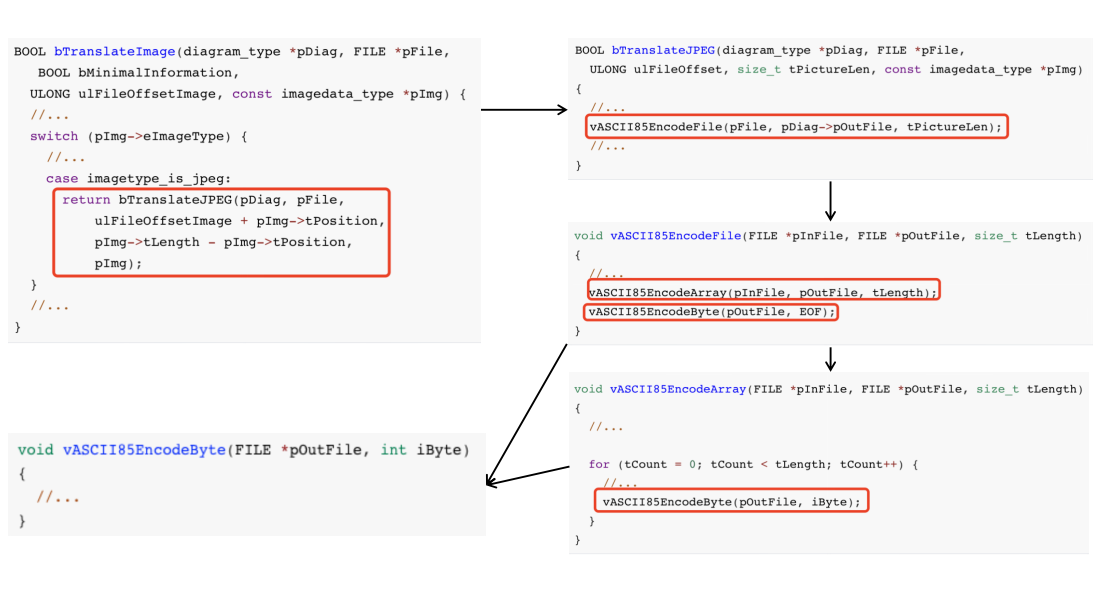
\includegraphics[width = 1\textwidth]{静态分析拒绝样例.jpg}
\caption{依赖闭包方法拒绝实例}
\end{figure}

(2)基于克隆代码接受率分析

基于克隆代码的方法的接受率最高,这表明克隆代码的特性与用户对变更传播的认知高度契合,进一步验证了本文假设:克隆代码一定程度上反映了变更影响关系。除此之外,我们还观察到部分未被接受的方法对存在一些特定的特征,进一步揭示了影响用户接受率的其他因素。

例如,以antiword项目中的一对包含克隆代码片段的方法为例,这两个方法的统计信息如表3-5所示,其中克隆代码片段仅占据8行。而这两个方法的克隆代码片段如图3-5所示,包含的重复代码仅为两行单独的语句。之所以在统计时被视为克隆代码,主要是由于编程习惯的影响,每个参数被单独放在一行,这导致了克隆代码的扩展至8行。用户认为此例较为牵强,因为克隆代码占整个方法的行数过少,这表明克隆代码所占比例可能是用户决定是否信任该项分析的重要因素之一,除此之外这一点可能也需在对代码进行预处理时,对代码格式进行统一,防止一句扩展成多行的情况发生。

\begin{table}[htbp]
\caption{包含克隆代码片段的方法实例统计信息}
\vspace{0.5em}\centering\wuhao
\begin{tabular}{cccc}
\toprule
方法 & 代码行数(Line of code)  & 克隆代码长度\\
\midrule
pHdrFtrDecryptor & 125 & 8 \\
szFootnoteDecryptor  & 115 & 8 \\
\bottomrule
\end{tabular}
\end{table}

\begin{figure}[h]
\centering
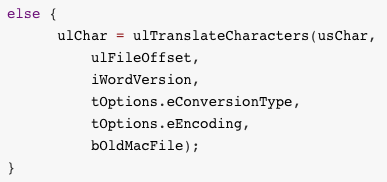
\includegraphics[width = 0.6\textwidth]{克隆代码片段.jpg}
\caption{克隆代码片段}
\end{figure}

(3)基于数据挖掘接受率分析

基于数据挖掘方法得到的接受率表现良好,均在60\%以上。这里选取了未被其他方法所检测到的正例样本,说明数据挖掘方法的优秀潜力。

以librdkafka项目中挖掘到的方法对为例,如图 2-6 中所示,这个项目是 kafka 的一个 C/c++客户端。方法一的主要功能是在 Kafka 模拟环境中按照一定的规则生成 Producer ID,而方法二的功能是检查一个 Producer ID 是否有效。当涉及检查的逻辑时,往往需要考虑到它是如何被创建和分配的。在这个例子中需要确保 ID 的创建逻辑与检查逻辑一致,才能确保检查是正确的。这个方法中,对于要检查的 Producer ID,首先会判断事务 ID,然后再检查 epoch,逻辑与创建 ID 是形成对应的。考虑修改的行为,如果对于 Producer ID 的创建和分配逻辑进行了修改,那么通常需要同时修改 Producer ID 检查逻辑,以确保两者保持一致。否则,如果创建和分配逻辑发生了变化,而检查逻辑没有相应地进行调整,就可能导致检查逻辑无法正确地验证新生成的 Producer ID,从而引入错误和不一致性。

\begin{figure}[h]
\centering
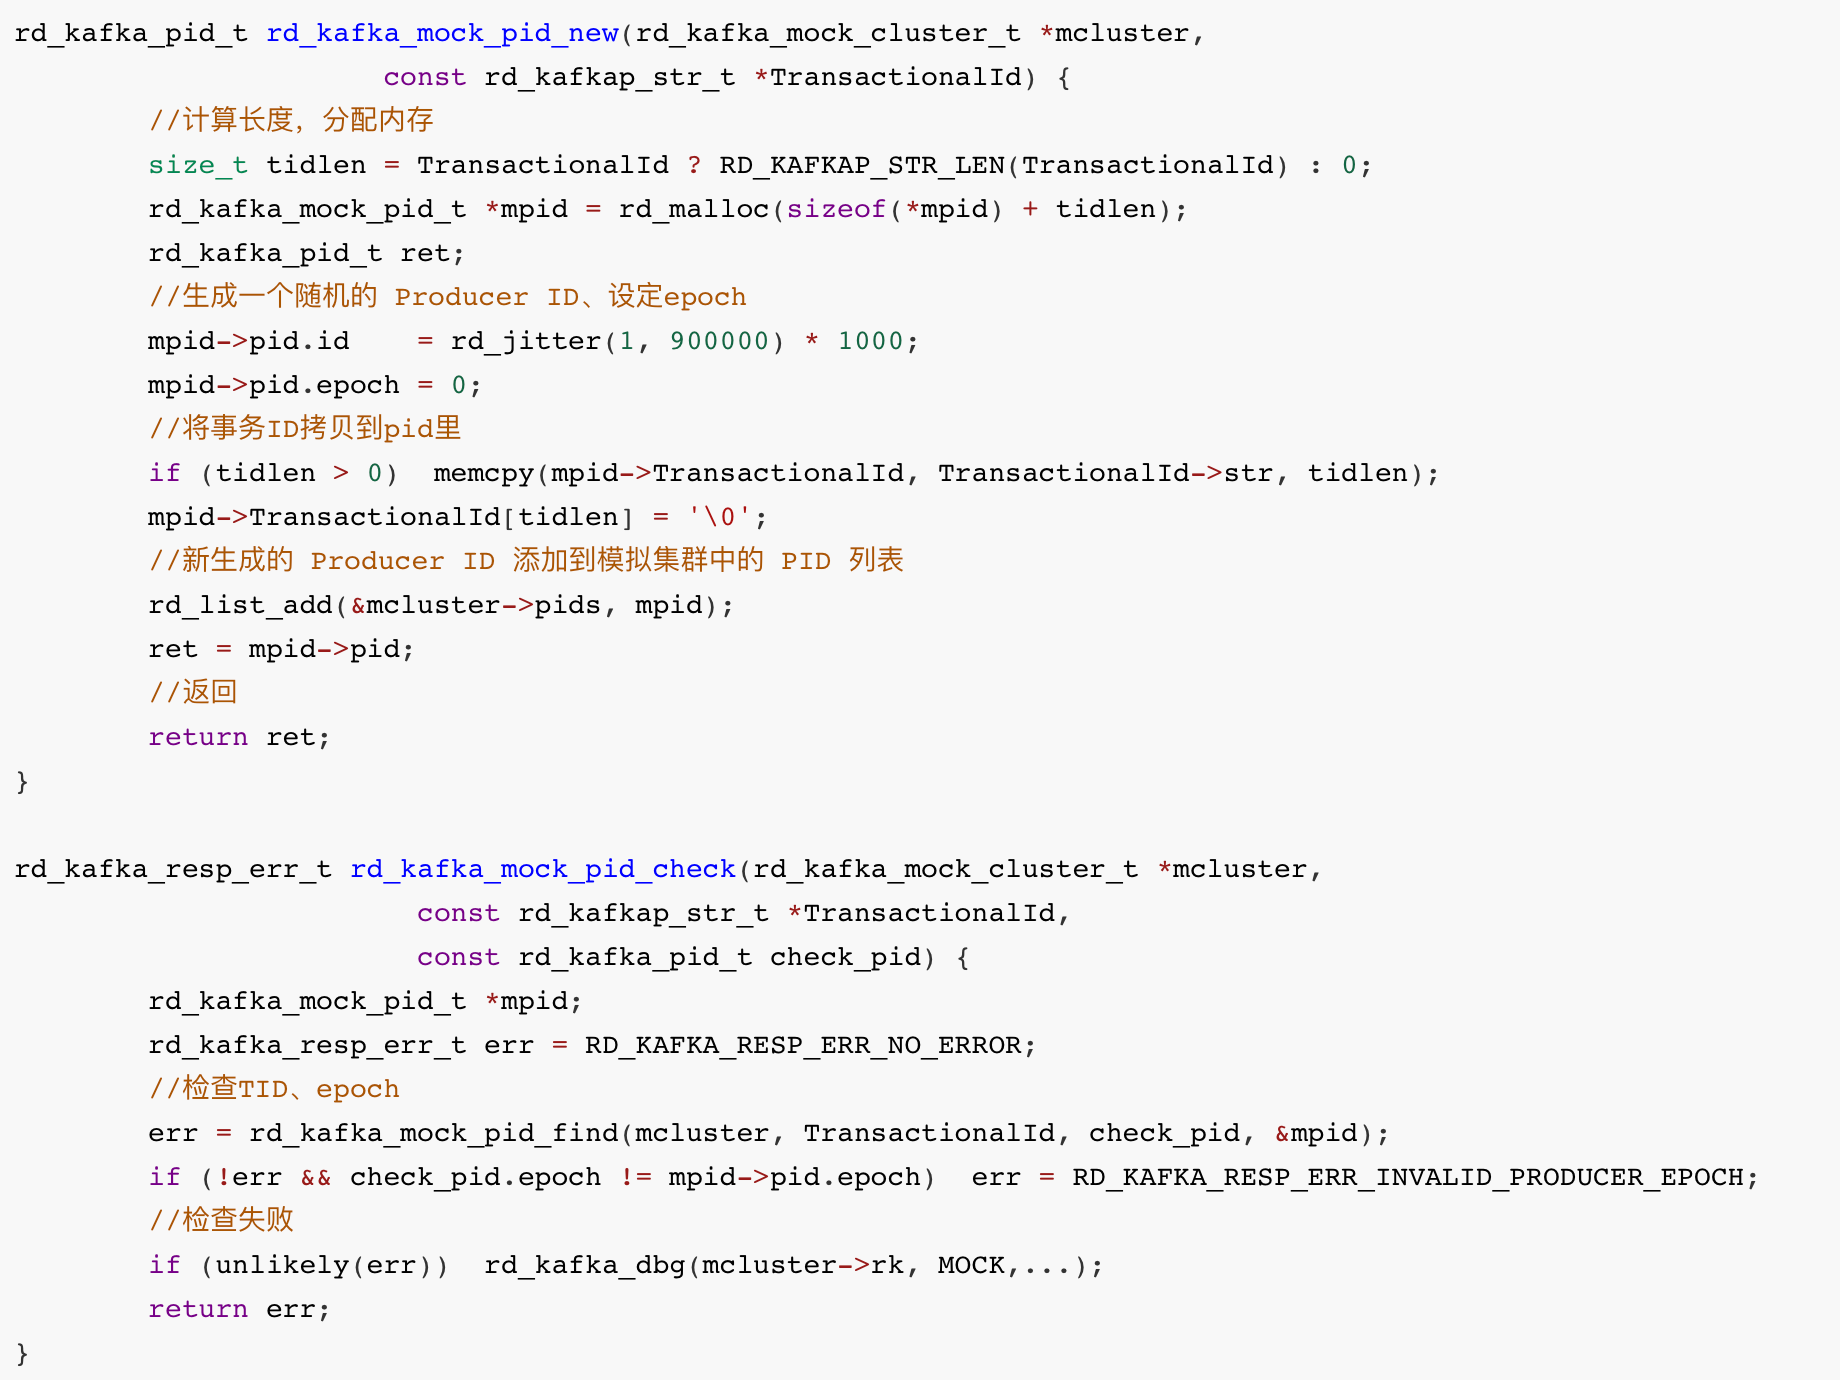
\includegraphics[width = 0.6\textwidth]{数据挖掘挖到的方法对.png}
\caption{逻辑上有变更影响关系的方法对示例}
\end{figure}

另一个更好理解的例子是push和pop方法对,这对方法在逻辑上是一定镜像的,push的操作必须和pop的操作一一对应,才能保证代码逻辑的正确性,这个例子同样仅被数据挖掘方法检测到。

\begin{figure}[h]
\centering
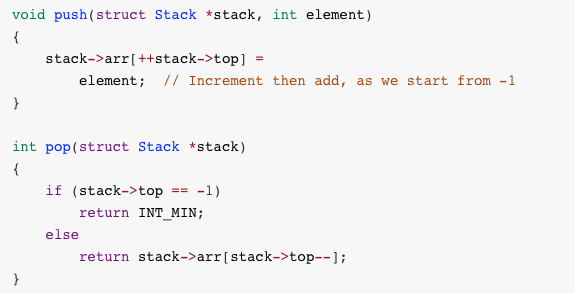
\includegraphics[width = 0.6\textwidth]{pushpop.jpg}
\caption{逻辑上有变更影响关系的方法对示例}
\end{figure}

经过分析可以看出,通过数据挖掘方法得到的具有变更关系的方法对,是具有一定的准确性的,并且可以弥补基于依赖闭包方法中仅关注调用依赖关系的不足。

\section{本章小结}

本章介绍了四种变更影响分析方法。

(1)传统的基于依赖关系闭包的变更影响分析方法。该方法首先对软件项目进行预处理,提取抽象语法树、方法摘要表和全局变量信息表等数据结构,然后构建依赖关系图,节点表示方法和全局变量,边表示方法之间的调用关系。然后根据依赖闭包对每个方法提取对应影响方法。

(2)基于克隆代码的变更影响分析方法。该方法认为代码克隆关系一定程度上反映了变更影响关系,通过ClaSP算法进行序列挖掘,提取代码克隆,从而反映变更影响关系。

(3)基于数据挖掘的变更影响分析方法。该方法认为代码变更历史蕴含了一定的变更影响关系,通过提取代码的提交历史,根据频繁模式挖掘理论,挖掘出频繁共现的方法对,从而反映变更影响关系。

(4)基于深度学习的变更影响分析方法。对不存在变更历史的项目,通过数据挖掘得到的数据整理成数据集,训练深度学习模型,对项目方法之间的变更影响关系进行预测。

最后,本章通过实验验证了四种方法在提取变更影响关系上的有效性,实验结果表明,除传统的基于依赖关系闭包的方法外,其他方法都取得了良好的检测效果。除此之外还通过实例分析,说明了每种方法的缺点和各自的侧重点。

%%%%%%%%%%%%%%%%%%%%%%%%%%%%%%%%%%%%%%%%%%%%%%%%%%%%%%%%%%%%%%%%%%%%%%%%%%%%%%%


\chapter{代码审查图生成}
\section{引言}


在软件开发过程中,开发者通常会经历多个阶段。在项目的初始阶段,开发者需要阅读和理解已有的代码,这是熟悉软件项目的第一步。然而,对于大型项目而言,由于项目代码量庞大,涉及的模块和功能众多,这一过程通常需要耗费大量的时间和精力。除此之外,开发者在对软件进行修改时,如添加新功能或修复缺陷,通常需要深入了解修改代码的上下文信息。如果对上下文理解不清晰,可能会导致变更不完全或不准确,进而影响软件质量。

在软件开发的后期,开发者往往需要作为代码审查者参与到代码审查过程中。代码审查的主要目的是评估变更后的代码是否符合质量标准,是否能够顺利地合并到主分支中。这一过程不仅在协作开发中至关重要,也是确保软件质量的有效手段。然而,代码审查往往需要投入大量的时间和精力\cite{花子涵2024代码审查自动化研究综述}。审查者不仅需要对变更的代码本身进行分析,还需要理解这些代码所处的上下文,才能做出正确的评估。

因此,无论是作为开发者还是审查者,理解软件项目的结构和代码是至关重要的。只有深入掌握软件的整体架构和各模块之间的关系,才能在后续的开发和审查过程中保证代码质量。然而,传统的代码阅读和理解方式不仅需要消耗大量的时间和精力,还难以确保高效性和准确性,尤其是在面对庞大复杂的代码库时。

为了提高代码理解的效率并减少人为错误,本文提出了一种基于代码审查图的代码质量分析展示方式。这一方法通过将项目中的各个方法和全局变量表示为图的节点,并用边表示方法与方法之间、方法与全局变量之间的依赖关系,从而形成一个结构化的代码关系图。这样的图形化展示方式能够帮助开发者和审查者从宏观的角度掌握整个软件项目的架构和各个模块之间的关系,进而提升对代码的理解效率。通过这种方式,开发者和审查者可以更直观地识别出项目中的关键部分及其相互依赖关系,从而在变更和审查过程中更高效地评估代码的质量和影响。

\section{基于标签生成的方法模块分类}
\subsection{基于大语言模型的方法模块标签生成}

在软件项目中,还有一项非常重要的设计因素就是项目的模块划分。在软件项目设计的最初,会根据功能、承担责任等角度将软件划分为多个模块,不同模块承担不同的责任,模块之间通过调用等依赖关系,共同实现功能。

模块有不同的实现方法,通常是将放在同一文件或同一文件夹内,通过模块命名来划分具有相同功能的代码。但是随着长时间的维护和开发,软件项目的架构往往会逐渐腐化,失去了最初设计的样子。这样还会导致某些代码错误地归属了某些模块,耦合度增加,牵一发而动全身,项目更加难以维护。对于这样的项目,重构往往成了唯一的手段。

而重构首先就需要对代码块所属模块进行辨认,相当于给代码块贴标签,标志其所属的模块的功能。现有的方法通常是基于耦合关系,通过聚类的方式\cite{2017Extraction},将联系紧密的方法聚为一类,提取为单独的模块。这种方法属于无标签的聚类,仅依赖耦合关系对模块进行划分。但是,实际上软件项目的模块恰恰不是无监督的,最初的模块设计通常是良好的且有逻辑的,只是后期的维护导致这种结构退化了,因此代码最初的模块就是标签。而无标签的聚类方法相当于认可了后期恶化的结构,这并不符合代码模块设计的初衷。

因此本文认为,对代码进行模块划分,应包含两个标签,一个是代码的原始标签,这个标签表示的当前代码所处功能模块名称,另一个是代码的随着代码的维护现在应在的实际模块名称,称为实际标签。首先应根据模块设计和代码的实际功能来对代码生成实际标签,然后再按原始标签对代码进行聚类,聚类得到的一类中,如果有实际标签不属于本模块的,则认为该方法应与原模块进行分离,合并到实际模块中去。

因此首先需要对代码块的实际功能来对代码生成实际标签。本文代码块的研究粒度是方法,因此该问题进一步被描述为给定一个模块名列表和一个方法,根据方法功能判断该方法应属于哪个模块。

由于大语言模型的较强的理解和推理能力,并且经过验证,大模型具有良好的文本分类效果\cite{wan-etal-2023-gpt},而大模型对于代码的理解不差于对文本的理解,因此本文尝试使用大语言模型进行分类。研究方案如下

\begin{figure}[h]
\centering
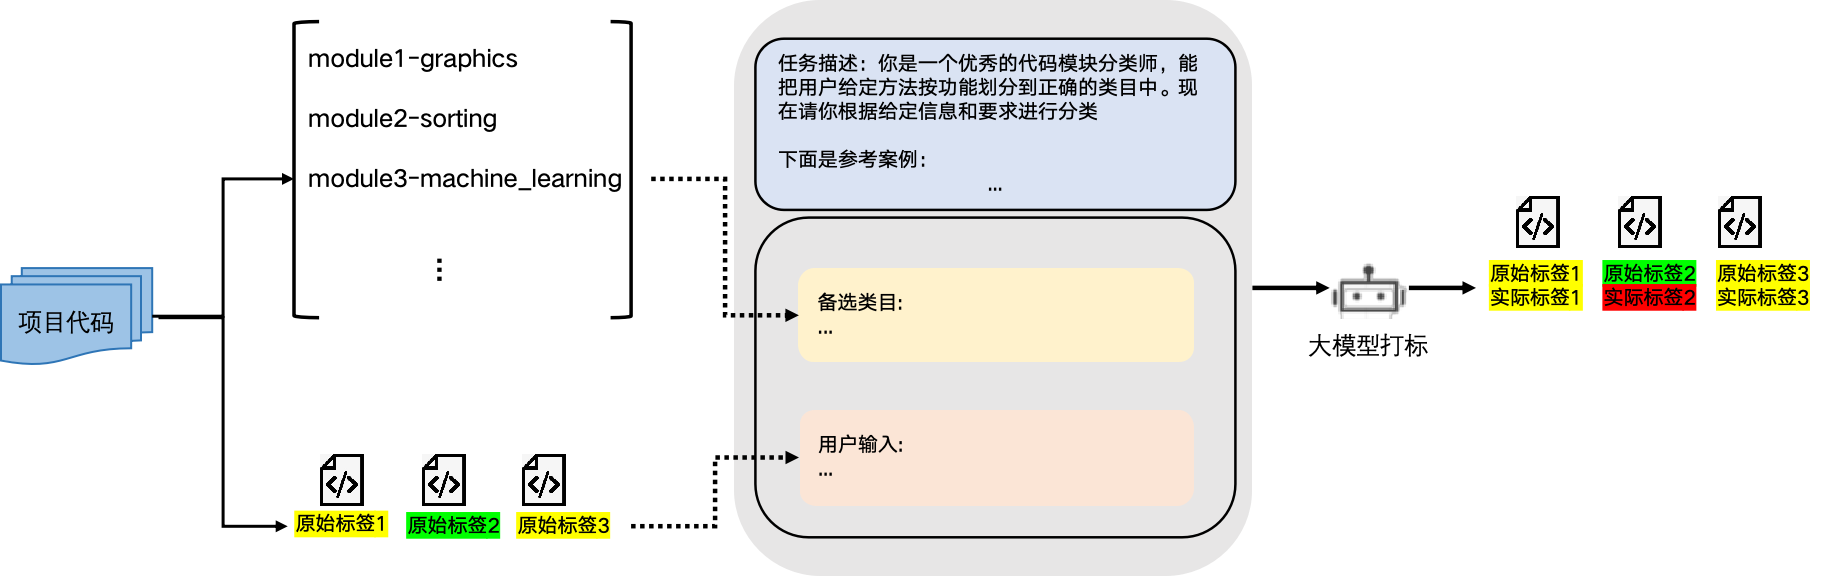
\includegraphics[width = 0.8\textwidth]{大模型预测.png}
\caption{逻辑上有变更影响关系的方法对示例}
\end{figure}

首先从项目代码中提取所有模块名,作为备选类目,提取方法的原始模块名并记录原始标签,将方法和备选类目组织成任务的描述,送给大模型进行打标,让其根据方法本身的功能,对方法进行分类打标,得到方法的实际标签。


\subsection{基于原始标签的方法分类}

大模型打标得到实际标签后,按项目的模块对方法进行分类。将模块名作为类别名,创建对应的一个个集合。遍历每一个方法,按方法的原始标签将方法放入对应的集合,完成分类。

\begin{figure}[h]
\centering
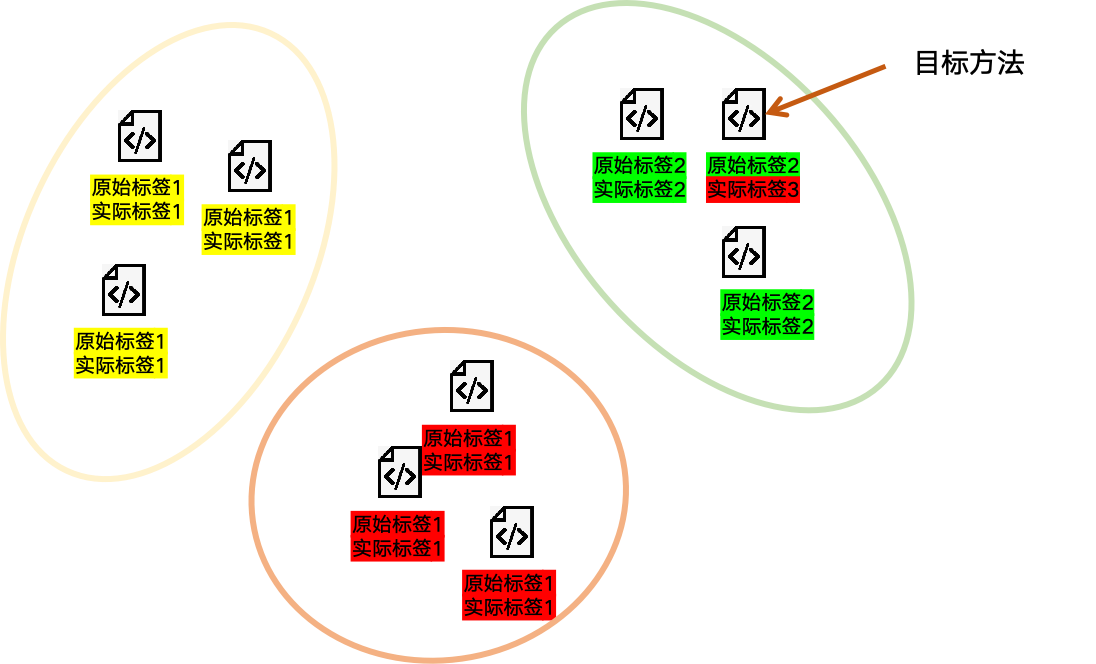
\includegraphics[width = 0.6\textwidth]{分类示例.png}
\caption{逻辑上有变更影响关系的方法对示例}
\end{figure}

分类结束后,我们会观察到这样的现象,每一个模块对应的方法列表中,会有实际标签并不是该模块的方法,这说明该方法是在代码维护过程中,被退化过程所影响的方法,用户应进一步观察该方法是否应在拆分到实际模块中。


\section{代码审查图}

\subsection{代码审查图构建}

代码审查图主要由两个核心元素构成,即节点和边。其中,节点代表软件项目中的方法或全局变量,边则表示节点之间的各种关系,如耦合关系、变更影响关系以及依赖调用关系。这些元素的结合能够帮助开发者从全局视角理解和评估项目的结构和质量,尤其是在进行代码审查和变更分析时。

(1)节点属性

在代码审查图中,节点的作用是标识项目中的方法和全局变量。通过前文所述的方法摘要表和全局变量信息表,我们为每个方法和全局变量创建了对应的节点。每个节点都具有多个属性,这些属性能够提供有关节点所代表的方法或变量的关键信息,便于开发者对代码进行全面的审查和分析。

对于方法的属性,通常可以分为两个主要部分:

首先是方法的基本信息,如表4-1所示。这一部分包括方法的名称、所在模块、方法签名、访问修饰符等基本信息,这些信息有助于开发者快速识别和定位方法的功能和作用。例如,方法的名称可以反映其业务功能,所在模块和调用信息则有助于理解方法的上下文和调用约束。


\begin{table}[htbp]
\caption{代码审查图节点属性-基本信息}
\vspace{0.5em}\centering\wuhao
\begin{tabular}{cccc}
\toprule
 属性 & 描述 \\
\midrule
方法名 & 方法名,由方法所在路径和方法名拼接而成,保证唯一  \\
方法参数 & 方法的参数列表,包括参数的名称和类型   \\
方法内调用方法 & 本方法内调用的其他方法名   \\
方法可作用域 & 表明方法是否全局可用   \\
方法所在模块 &  方法所在模块,目前表示为方法所在文件  \\
模型预测方法模块 & 模型预测的方法应在的模块   \\     
\bottomrule
\end{tabular}
\end{table}

其次是与代码质量相关的度量和信息,如表4-2所示。这一部分基于前文方法提取和统计结果,涵盖了一些与代码质量直接相关的指标,如方法的扇入扇出、内聚度、耦合性等。这些度量和指标的结果将结合项目的具体统计数据或检测结果,向开发者提供有针对性的改进建议。例如,如果某个方法的扇出度位居项目中的前5\%,则可能表明该方法在项目中的依赖关系过于复杂,可能导致高耦合性,进而影响系统的灵活性和可维护性。类似地,如果检测出某方法存在不良耦合,则可能需要开发者重新设计该方法与其他模块的接口,以减少不必要的依赖。

\begin{table}[htbp]
    \caption{代码审查图节点属性-质量相关信息}
    \vspace{0.5em}\centering\wuhao
    \begin{tabular}{ccp{9cm}}
    \toprule
    属性类别 & 属性 & 描述 \\
    \midrule
    \multirow{2}{*}{扇入扇出信息}& 扇入 &  方法的扇入值以及扇入值在项目中的排名比例 \\       
                                & 扇出 &  方法的扇出值以及扇出值在项目中的排名比例 \\   \cline{2-3}
    \multirow{2}{*}{内聚度信息}& LCOM1 &  所在模块的LCOM1值以及相应建议 \\       
                                & LCOM2 &  所在模块的LCOM2值以及相应建议 \\    
                                & LCOM3 &  所在模块的LCOM3值以及相应建议 \\    
                                & LCOM4 &  所在模块的LCOM4值以及相应建议 \\    
                                & TCC &  所在模块的TCC值以及相应建议 \\    
                                & LCC &  所在模块的LCC值以及相应建议 \\   \cline{2-3}             
    \multirow{2}{*}{耦合关系}& 数据耦合 &  与本方法存在数据耦合关系的方法 \\       
                                & 标记耦合 &  与本方法存在标记耦合关系的方法 \\   
                                & 外部耦合 &  与本方法存在外部耦合关系的方法 \\   
                                & 公共耦合 &  与本方法存在公共耦合关系的方法 \\   \cline{2-3}
    变更影响关系 & 变更影响关系 &  与本方法存在变更影响的方法,表明来源为代码克隆、变更历史、模型预测 \\    \cline{2-3}
    缺陷 & 静态代码缺陷 &  由cppcheck检测得到的本方法缺陷 \\      
    \bottomrule
    \end{tabular}
    \end{table}

对于全局变量的属性则主要包含表4-3中的信息。主要是对全局变量基本信息的展示,方便开发者快速了解该变量的作用域、使用情况以及与其他代码部分的关联性。通过这些信息,开发者能够更好地理解变量在整个项目中的作用及其潜在的质量风险。

\begin{table}[htbp]
\caption{代码审查图节点属性-全局变量信息}
\vspace{0.5em}\centering\wuhao
\begin{tabular}{cccc}
\toprule
    属性 & 描述 \\
\midrule
变量名 & 全局变量名,由所在路径和变量名拼接而成,保证唯一  \\
变量类型 & 变量类型   \\
被使用方法 & 使用了本全局变量的方法名   \\
变量可使用域 & 表明变量是否全局可用   \\
方法所在模块 &  变量所在模块,目前表示为所在文件  \\  
\bottomrule
\end{tabular}
\end{table}


(2)边的设计

在代码审查图中,边表示节点与节点之间的关系,这些关系揭示了软件系统中各个方法与全局变量之间的相互依赖和影响。根据其性质,边的类型主要分为三类,具体分类如表4-4所示:静态依赖关系、耦合关系和变更影响关系。

其中静态依赖关系分为方法之间的调用关系和方法与全局变量的使用关系,耦合关系如表4-2中所示共4类,变更影响关系则根据检测方法的不同,设定为3个不同的来源。需要注意的是,由于依赖闭包方法本身是基于依赖图生成的,因此在代码审查图中,这类关系不再单独指出。

每种关系反映了不同层次的代码相互作用,帮助开发者全面理解系统的结构和潜在的质量风险。

\begin{table}[htbp]
\caption{代码审查图边分类}
\vspace{0.5em}\centering\wuhao
\begin{tabular}{cccc}
\toprule
属性 & 描述 \\
\midrule
静态依赖关系 & 含方法之间调用、方法使用全局变量两种  \\
耦合关系 & 含数据耦合,标记耦合,外部耦合,公共耦合四种   \\
变更影响关系 & 含代码克隆、变更历史、模型预测三种  \\
\bottomrule
\end{tabular}
\end{table}



\subsection{代码审查图可视化}

本节从代码审查图的可视化方案和交互方案两个方面展开介绍。

1.可视化方案 

代码审查图的可视化方案基于开源项目 G6。G6 是一个强大的图形可视化引擎,提供了绘制、布局、分析、交互、动画等全方位的图形可视化基础功能,具有简单易用且完备的特性。G6 具有两个显著优势。

(1)数据与可视化图形分离:在使用 G6 时,用户只需将图的数据组织为 JSON 格式,如图4-1所示,包括节点信息和边信息,直接传递给 G6 即可自动生成对应的力导向图。这种数据与图形的分离不仅简化了开发流程,还提高了数据的灵活性和可操作性,便于进行后续的数据更新和图形重绘。

\begin{figure}[h]
\centering
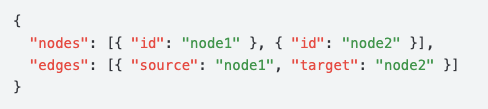
\includegraphics[width = 0.6\textwidth]{G6图数据示例.jpg}
\caption{G6图数据示例}
\end{figure}

(2)高度的定制能力:G6 提供了丰富的图形展示配置选项,用户可以根据需求自由选择不同的样式和布局方式。如果 G6 内置的元素不满足特定需求,它还支持用户自定义节点、边及其他元素,使得图形展示更加贴合实际应用场景。

本文使用G6内置节点和边实现代码审查图的可视化。G6的节点构成共包含6部分,其中label表示文本标签,通常用于展示节点的名称或描述,本文中将节点属性赋值给label,便于用户查看属性相关信息。G6的边的构成共包含4部分,label具有同样的功能,将边的类别用于label。让 G6 加载此数据源进行展示,就实现了同时也实现了计算逻辑与图形可视化的有效分离。


2.交互方案

对于软件项目这样的分析对象,方法和全局变量的数量常达到千级别,这样的级别对于一个图来讲,很难在图中展示完所有的信息,因此需要用户交互,来展示更详细的信息。表 2-8 展示了目前代码审查图的交互和对应的逻辑设计。




\begin{table}[htbp]
\caption{代码审查图交互和逻辑设计}
\vspace{0.5em}\centering\wuhao
\begin{tabular}{cccc}
\toprule
交互方式 & 业务逻辑 \\
\midrule
视角缩放 & 操作鼠标滚轮对图进行缩放  \\
视角移动 & 鼠标拖拽移动整个代码审查图   \\
聚焦节点 & 光标悬停在节点上显示节点的方法名/变量名  \\
移动节点 & 鼠标长按节点拖拽可移动节点 \\
查看节点属性 & 鼠标点击节点展开节点属性  \\
聚焦关系 & 光标悬停在边上显示边的类型  \\
查看关系信息 & 鼠标点击节点展开节点属性  \\
节点筛选 & 通过点击筛选节点按钮,确认是否筛选掉孤立节点 \\
边筛选 & 通过选择不同类型的关系,筛选掉其他类型 \\
节点搜索 & 通过搜索方法名/变量名,高亮对应节点  \\
\bottomrule
\end{tabular}
\end{table}



\subsection{代码审查报告生成}

在软件开发过程中和审查过程中,用户可通过代码审查图聚焦关注代码的上下文,但当软件开发完成,想总体衡量软件项目的质量时,仅依靠代码审查图,同样会有质量信息过于分散,不好聚焦的问题。因此这里通过生成文档形式的代码审查报告,交给开发者进行统一的代码质量概览。

代码审查报告的主要内容是报告软件项目中存在的质量问题,分为部分。报告的粒度分为两方面,一种是模块级别,另一种是方法级别。

模块级别包括模块的内聚度信息,这里会报告用户那些内聚度为最差的5\%的模块,并给出相应的统计信息。除此之外还包括了大模型预测聚类后,标签不属于该模块的方法名称,交给用户判断是否该方法应与该模块分离,划归另一模块。

方法级别的信息包括代码缺陷信息,扇入扇出、耦合信息、代码变更影响信息,这里会报告方法中的静态检测工具检测出的代码缺陷、扇入扇出为最差的5\%的模块,不良的耦合信息和代码变更影响列表。

通过整合这些信息,供用户查阅,以了解整体的代码质量情况。

\section{实验结果与分析}

\subsection{实验环境与评价方法}
(1)实验环境

实验环境如表4-6所示。

\begin{table}[htbp]
\caption{实验环境}
\vspace{0.5em}\centering\wuhao
\begin{tabular}{cccc}
\toprule
    环境 & 信息 \\
\midrule
操作系统 & macOS Ventura v13.5.2  \\
Intellij pycharm & 2021.1.1   \\
python & 3.7   \\
Java & 1.8   \\
G6 & g6.min.js 4.3.11  \\  
libclang & 15.0.7  \\ 
pycparser & 2.21  \\
\bottomrule
\end{tabular}
\end{table}

本文使用了Doubao-lite-4k-240828、Doubao-lite-32k-240828、Spark Lite共三种大语言模型进行实验。

(2)评价方法

本章使用表2中的项目为示例项目。

对于基于标签生成的模块分类方法,我们首先需要验证大模型进行方法模块分类的准确性,只有当分类准确时,才能信任其对于方法拆分的建议。虽然没有真实标签,但是项目中的大部分方法都应属于原始标签,因此本文首先计算预测的实际标签和原始标签相等的比例。如果比例较高,则说明大模型预测模块有一定准确性,则进一步实例分析实际标签和原始标签不同的案例,验证其可行性。

对于代码审查图生成方法,首先对示例项目生成代码审查图,验证可视化方案的需求,根据代码审查图分析前文中实验结果,以说明代码审查图相较文字的优越之处。

对于代码审查报告的生成,

\subsection{实验结果与分析}

1. 大语言模型模块分类实验结果

示例项目中,预测的实际标签和原始标签相等的比例如表4-7所示。


\begin{table}[htbp]
\caption{变更影响接受率实验结果}
\vspace{0.5em}\centering\wuhao
\begin{tabular}{cccc}
\toprule
项目名称 & Doubao-lite-4k-240828 & Doubao-lite-32k-240828 & Spark Lite \\
\midrule
antiword & 66.2 & 73.4 & 43.1 \\
librdkafka & 42.1 & 45.3 & 33.7 \\
TheAlgorithms & \textbf{84.2} & 87.2 & \textbf{63.2} \\
libbpf & 83.7 & \textbf{96.2} & 53.1 \\
FFmpegKit & 40.6 & 57.7 & 31.7 \\
jemalloc & 60.6 & 60.3 & 39.8 \\
\bottomrule
\end{tabular}
\end{table}

总的来讲,实际标签和原始标签相等的比例并不低,有的项目甚至可达90以上,这说明大部分的方法实际标签等于原始标签的假设是有一定可信度的。单项目内横向对比,可以发现Doubao-lite-32k的比例大于Doubao-lite-4k,两个模型的比例都高于SparkLite,这可能是由于模型的性能问题。

为了使模块拆分的建议更具可信性,选择准确率较高的TheAlgorithms项目进一步分析。首先经过分析可以发现,该项目的文件命名和方法命名非常准确,见名知义,因此模型预测都较为准确,由此可以看出,模块命名是否规范,对模块预测具有较强的影响。其次对Doubao-lite-32k-240828模型预测的实际和预测并不相等的例子进行抽样分析,共167个方法,抽取其中50个方法进行分析,用户共接受了7个方法,接受率14.0\%,并不高。但是通过用户接受的例子也能发现,该方法有一定的实际意义。

\begin{table}[htbp]
\caption{TheAlgorithms项目中预测与实际不符的实例统计}
\vspace{0.5em}\centering\wuhao
\begin{tabular}{cccc}
\toprule
预测与实际不符方法总数 & 抽样 & 用户接受 & 所占比例 \\
\midrule
167 & 50 & 7 & 14.0\% \\
\bottomrule
\end{tabular}
\end{table}


2. 代码审查图

(1)代码审查图概览

如图表示分别是antiword项目和TheAlgorithms的代码审查图,图中圆形节点表示方法,方形节点表示全局变量。蓝色边表示依赖关系,绿色边表示耦合关系,红色边表示代码变更影响关系。上图是未区分模块的图,下图中将同一模块的染上相同颜色。

\begin{figure}[!h]
    \setlength{\subfigcapskip}{-1bp}
    \centering
    \begin{minipage}{\textwidth}
    \centering
    \subfigure[antiword代码审查图-未划分模块]{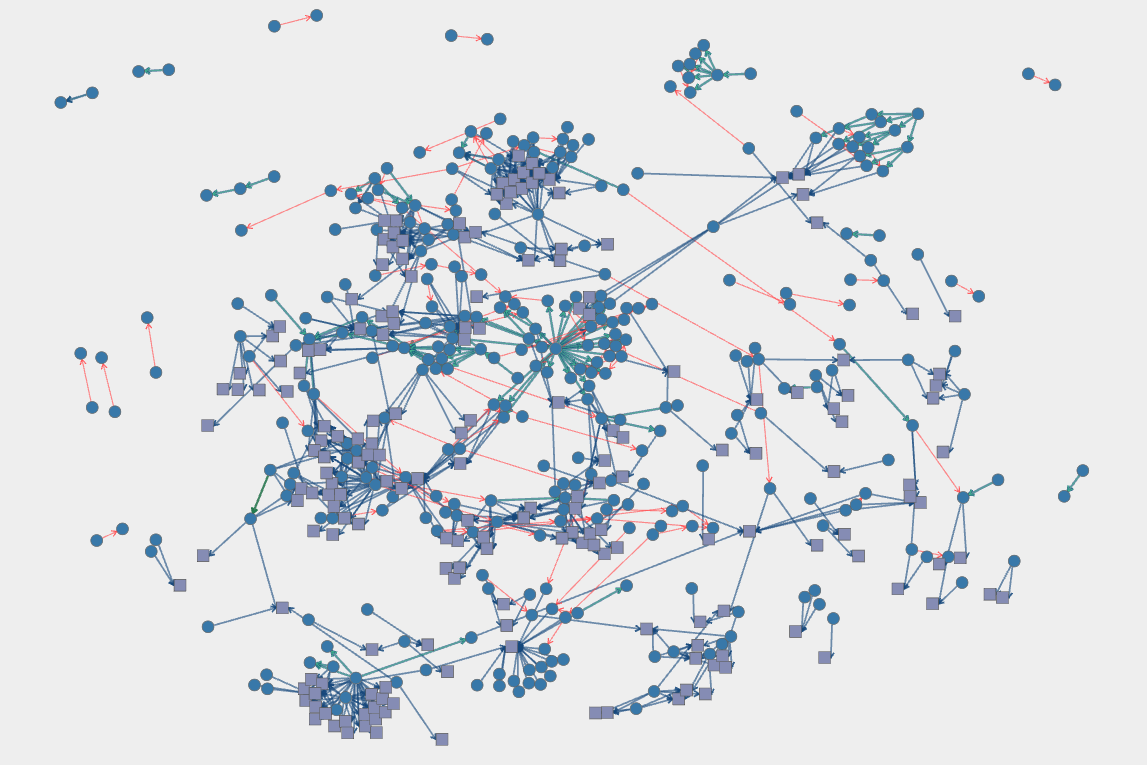
\includegraphics[width=0.4\textwidth]{antiword审查图未上色.jpg}} % 保留中文标题
    \hspace{2em}
    \subfigure[TheAlgorithms代码审查图-未划分模块]{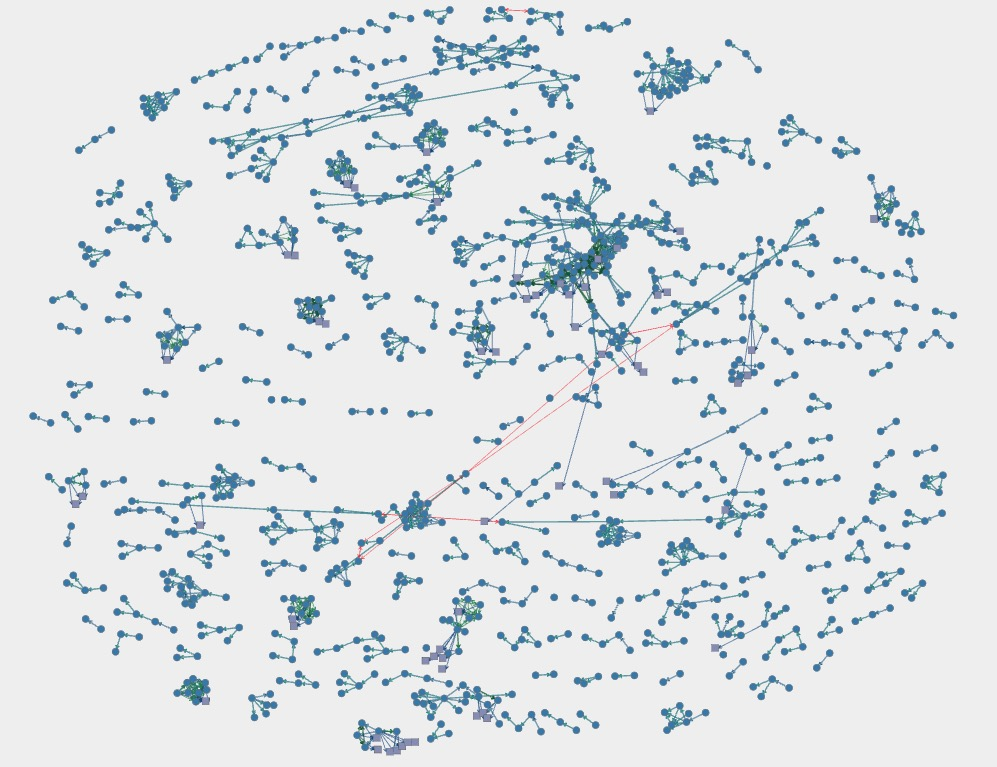
\includegraphics[width=0.4\textwidth]{aigri代码审查图-未上色.jpg}} % 保留中文标题
    \end{minipage}
    \centering
    \begin{minipage}{\textwidth}
    \centering
    \subfigure[antiword代码审查图-划分模块]{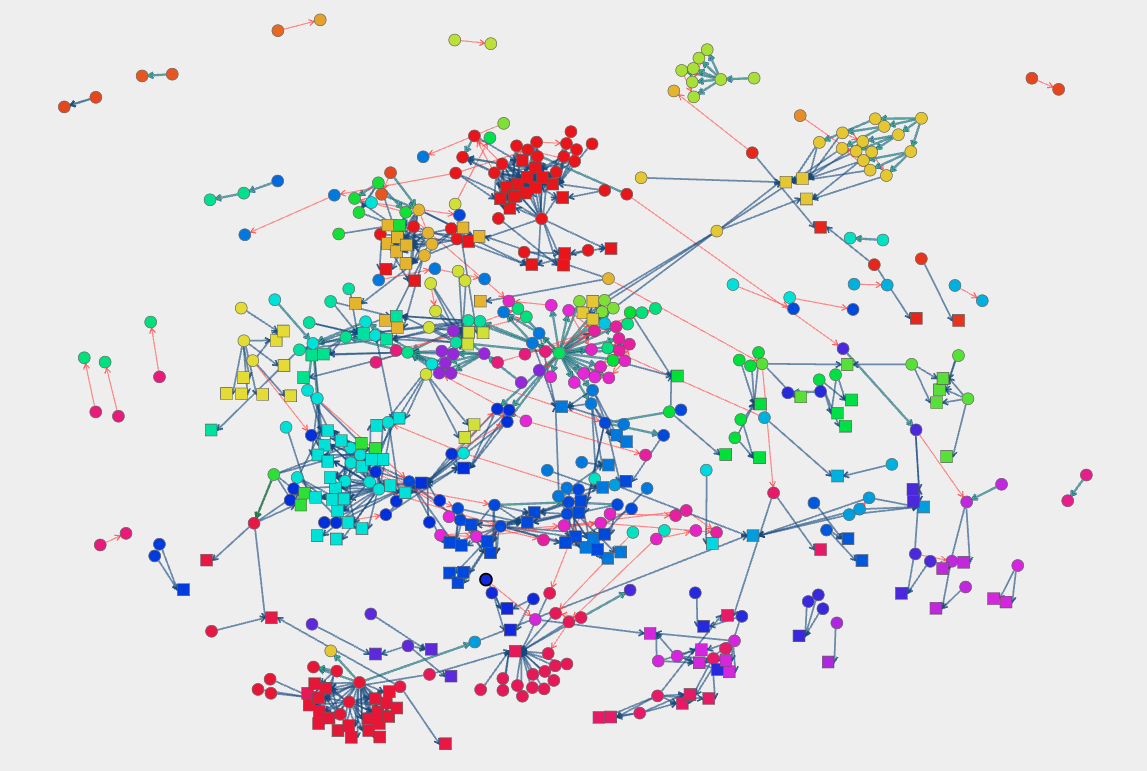
\includegraphics[width=0.4\textwidth]{antiword代码审查图.jpg}} % 保留中文标题
    \hspace{2em}
    \subfigure[TheAlgorithms代码审查图-划分模块]{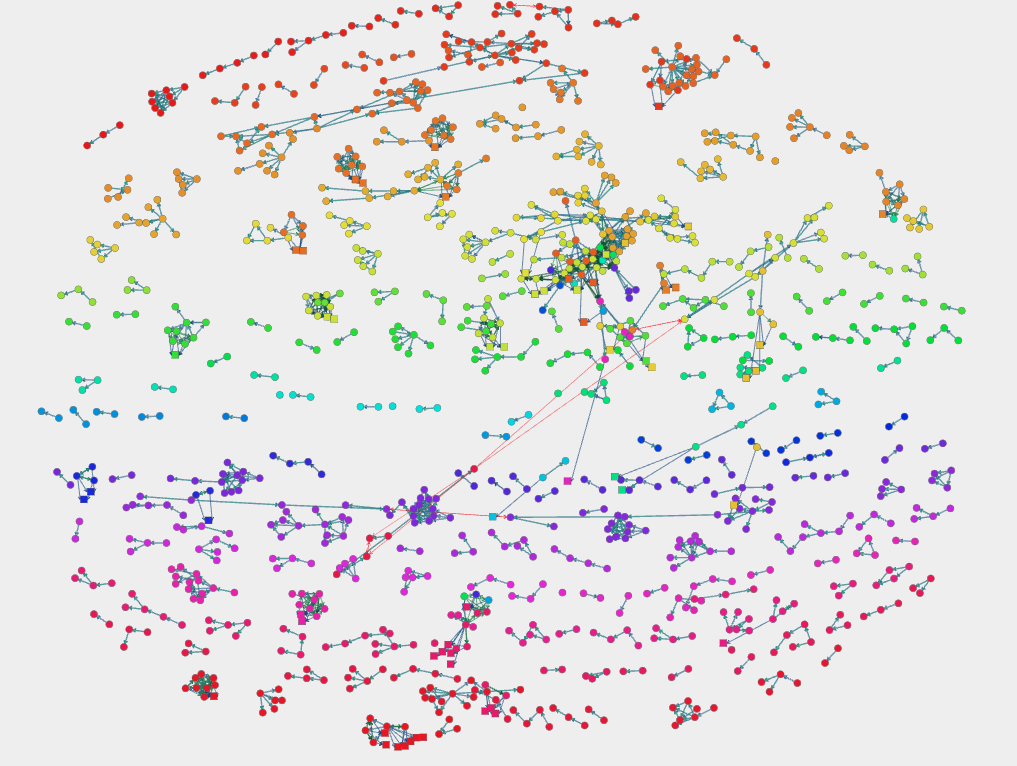
\includegraphics[width=0.4\textwidth]{aigri代码审查图.jpg}} % 保留中文标题
    \end{minipage}
    \vspace{0.2em}
    \caption{代码审查图} % 只保留中文标题
\end{figure}



根据图可明显看出两个项目的特征,antiword整个项目的各个模块相互协调,共同完成一个功能,因此模块之间的联系较多,整体结构耦合较为紧密,并且按所在模块划分可以发现,模块的聚集度是比较强的,表现为同一颜色的节点聚集在一起。而TheAlgorithms项目由于其库函数的特征,每个方法之间的耦合性并不强,每个模块之间的聚集程度也不够强,因此呈现为一个一个的分离模块,结构较松散。

点击某个节点,可以显示节点具体信息,帮助用户快速了解该方法或全局变量的详细信息。

\begin{figure}[h]
    \centering
    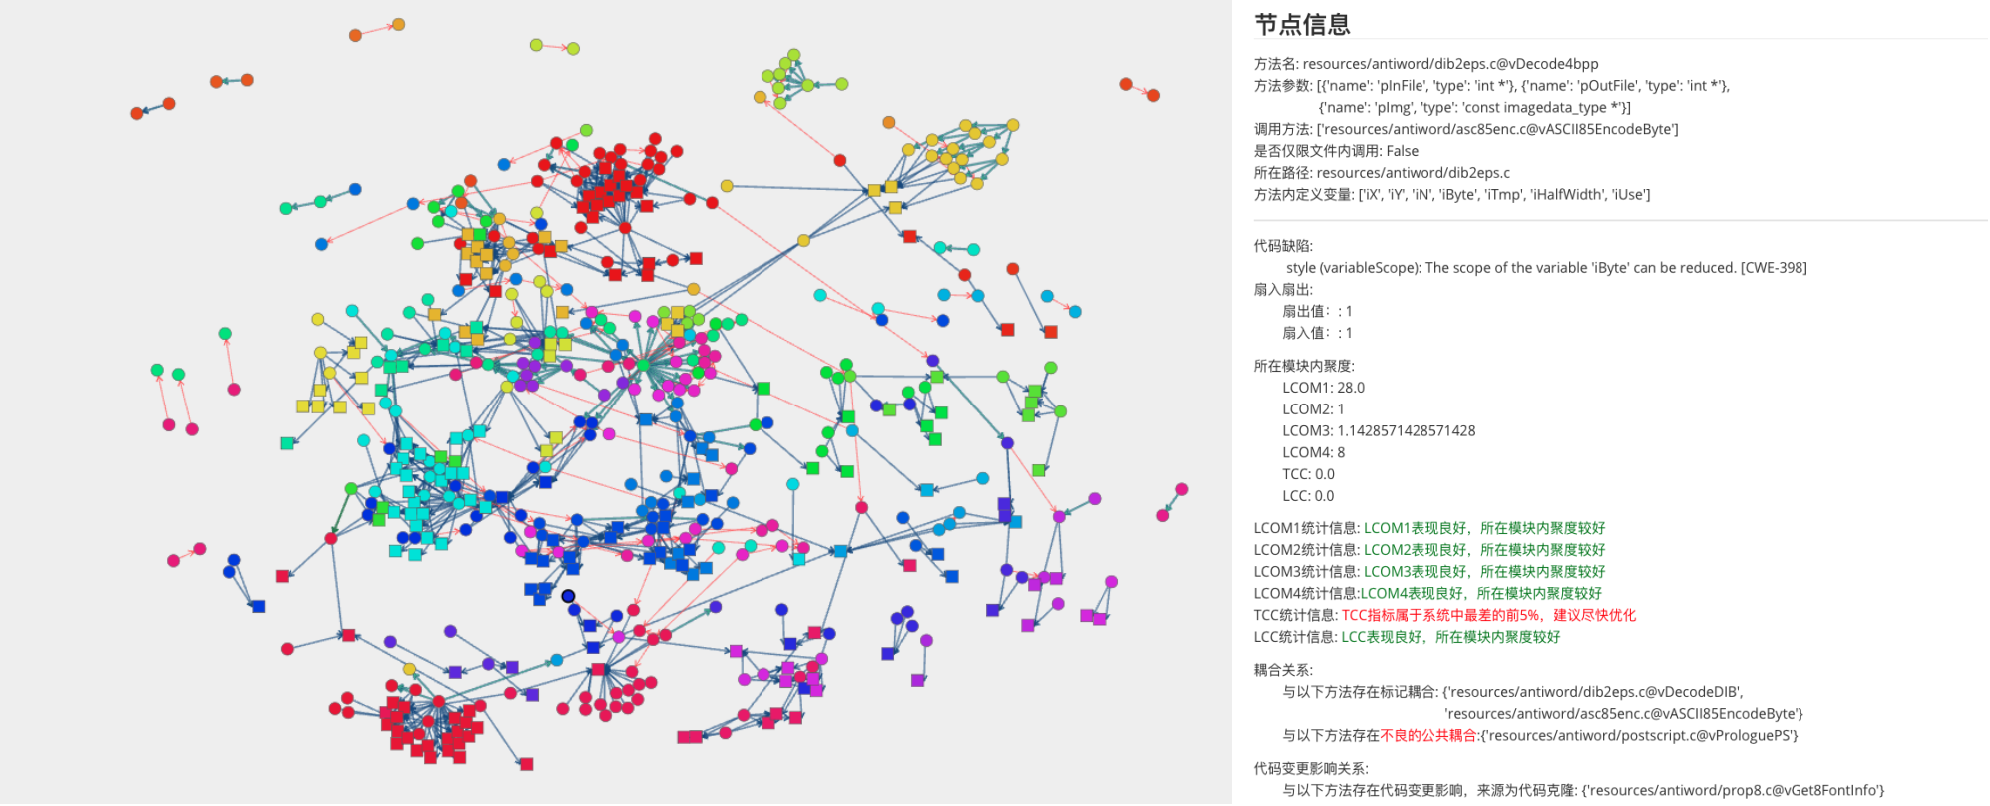
\includegraphics[width = 1\textwidth]{点击节点.png}
    \caption{点击节点展开节点信息}
    \end{figure}

(2)子图展示

这里以antiword项目中的子图为例。这个例子中我们聚焦vDecodeDIB方法,如果想对该方法进行开发,根据依赖关系和变更影响关系,我们至少需要阅读300+行代码,才能保证掌握了该方法的上下文逻辑,但是通过代码审查图,我们只需8个节点和9条边即可掌握。尤其是对于变更影响关系,这里指示了两个基于克隆代码的关系,作为开发者来说,这种关系是很难通过肉眼查看并记录的。因此可以发现,代码审查图对于开发者来说能够使其在阅读代码时,更直观地掌握代码间的各种依赖关系关系,在开发代码时,能帮助参考代码模块的关系,避免出现变更不完全的问题。而对于审查者来说,能够便于其快速理解上下文,和检查变更缺陷。

\begin{figure}[h]
    \centering
    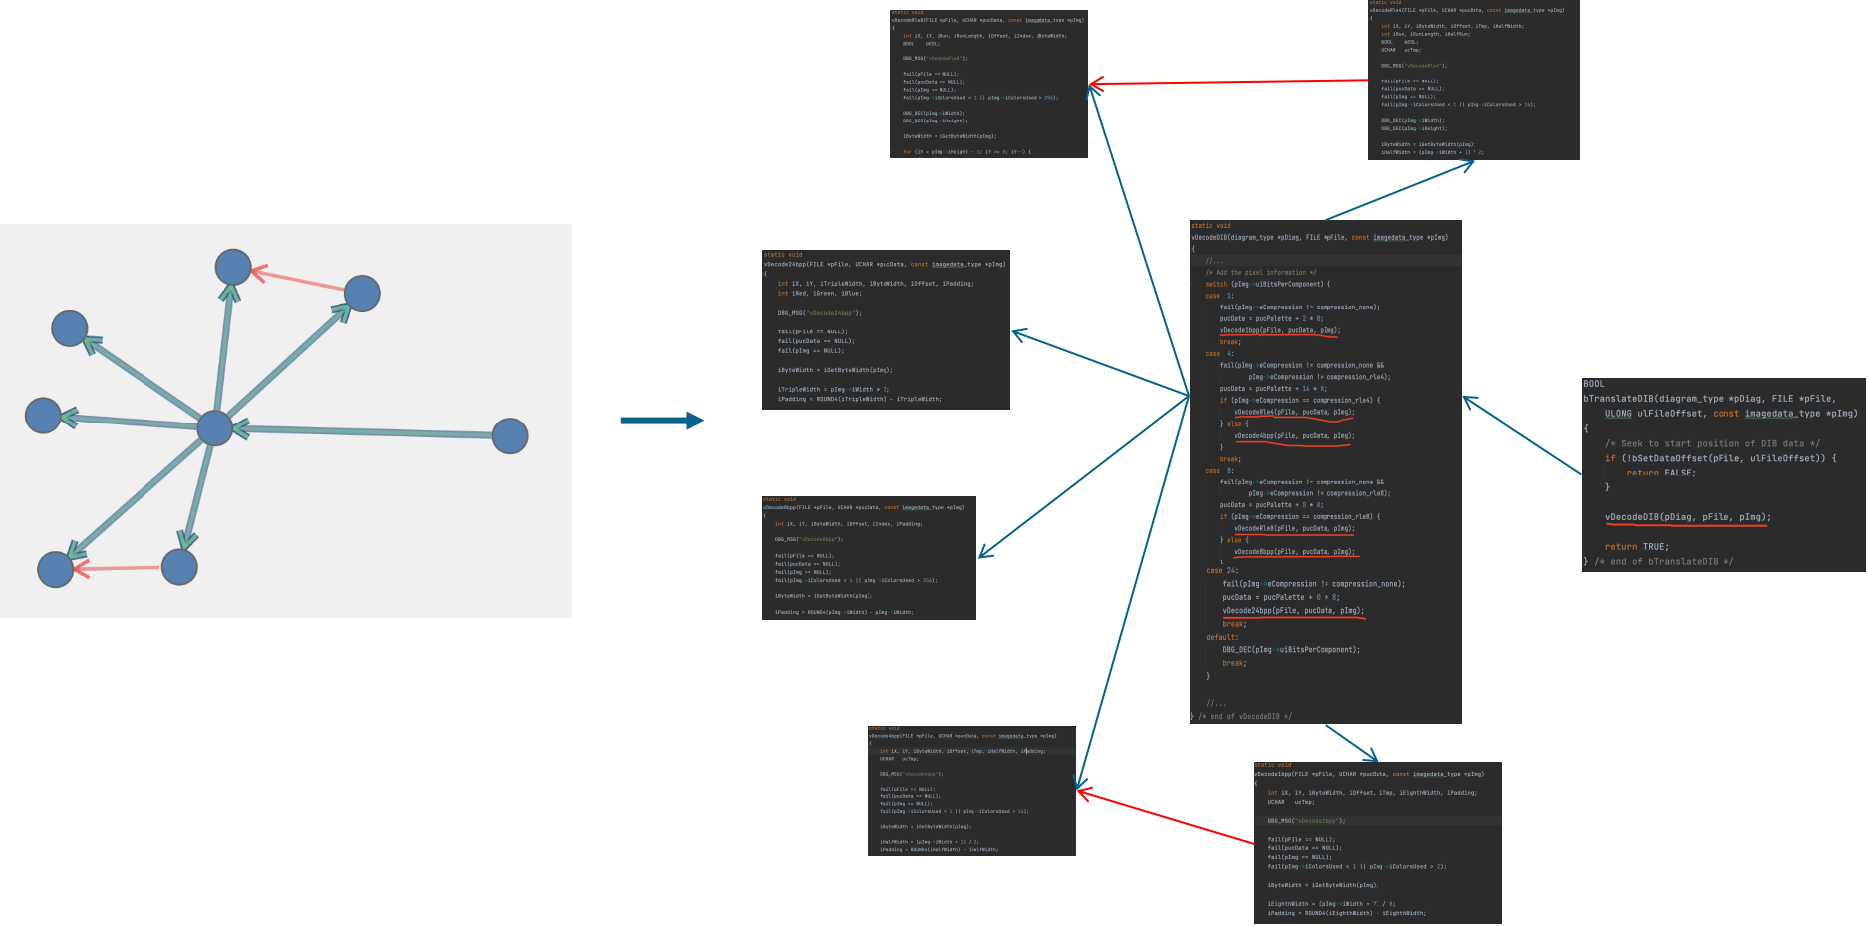
\includegraphics[width = 1\textwidth]{子图.png}
    \caption{vDecodeDIB方法上下文}
    \end{figure}

(3)代码特征体现

通过代码审查图,还能体现代码特征,辅助用户理解代码质量较差的原因。

在2.6.2节中,解释了misc.c 文件内聚度表现最差的原因,统计了其内部方法和变量的信息,但仅靠文字说明依旧不够直观,其对应的代码审查图如图所示,能清晰地反映出该模块的结构,不仅结构松散,还存在很多孤立节点,因此内聚度最差。

\begin{figure}[h]
\centering
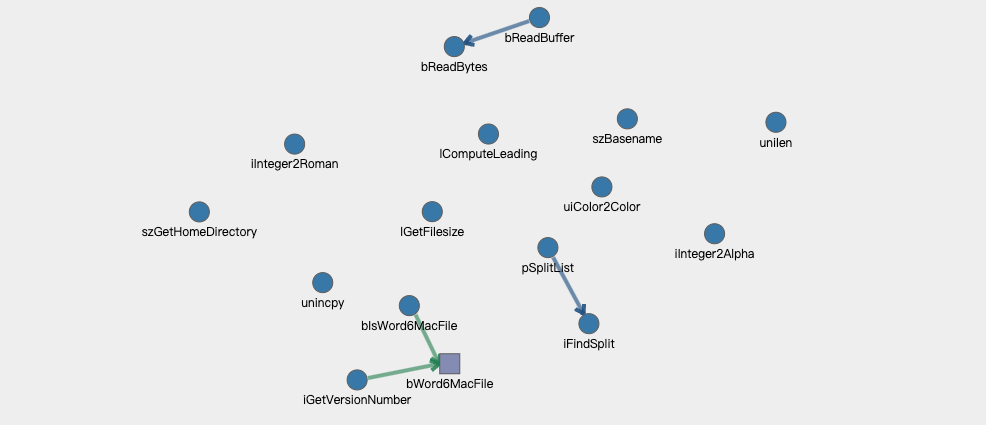
\includegraphics[width = 0.6\textwidth]{内聚度差例子.jpg}
\caption{misc.c 文件对应的代码审查图}
\end{figure}

再比如2.6.2节中对于高扇出方法的阐述,高扇出通常意味着方法复杂性过高,这样的特征在代码审查图中能非常明显地显示出来,用户可迅速通过代码审查图定位到对应的方法,了解其上下文,对不合理的高扇出做出相应的调整。

\begin{figure}[h]
\centering
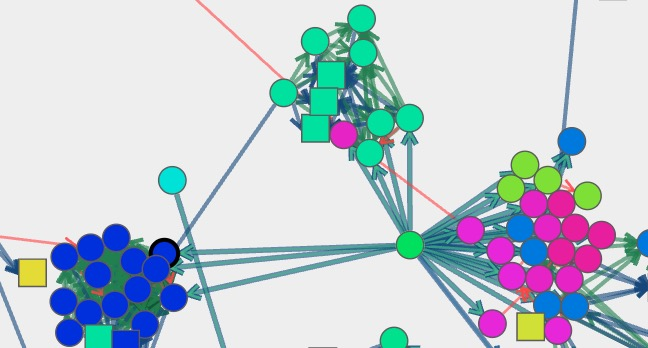
\includegraphics[width = 0.4\textwidth]{扇出度最高.jpg}
\caption{misc.c 文件对应的代码审查图}
\end{figure}


3. 代码质量检测报告

下图是代码检测报告的结构,图是实际的检测报告的一部分,通过代码检测报告,用户能以清单的方式了解软件项目的所有质量缺陷。



\section{本章小结}

本章介绍了基于标签生成的方法模块分类,该方法通过大语言模型生成方法的实际标签进行分类,表明模块划分不正确的方法,通过实验证明,该方法具有一定的参考意义。其次介绍了代码审查图,将软件分析结果以图的形式展示给用户,方便用户从宏观的角度了解项目结构,最后介绍了代码质量报告的生成,通过清单式的质量信息报告,方便用户查询和优化。





% Local Variables:
% TeX-master: "../main"
% TeX-engine: xetex
% End:
